\documentclass[a4paper,11pt]{scrartcl}

\usepackage[english]{babel}
\usepackage{pstricks}
\usepackage{graphicx}
\usepackage{supertabular}
\usepackage{caption}
\captionsetup{format=plain}
\usepackage{amsmath,amssymb,latexsym,mathtools} %Mathe
\usepackage{isomath}                            %nicht-kursive griechische Buchstaben
\usepackage{pifont}
\usepackage{caption, booktabs}
\usepackage{float}
\usepackage{extarrows}                          %Pfeile in den Formeln
\usepackage{siunitx}                            %SI-Einheiten
\usepackage{color, colortbl}                              %Farbige Texte
\usepackage{pdfpages}                           %PDFs einfügen für den Anhang
\usepackage{listings}                           %Aufzählungen
\usepackage{chemmacros}                         %--Allgemeines Chemiepackage--
\usepackage[version=4]{mhchem}                  %Chemische Reaktionsgleichungen
\usepackage{tikz, pgfplots}   
\usepackage{chemfig}                            %Chemische Strukturformeln
\usepackage{hpstatement}                        %P-H-Sätze
\usepackage{tabularx}
\usepackage{framed}  %PDFs mit Rahmen
\usepackage{xcolor}
\usepackage{mdframed}
\usepackage{cancel}
\usepackage{epstopdf}
\usepackage{longtable}
\usepackage{alphabeta}
\usepackage{esint}
\usepackage{bbm}
\usepackage{textgreek}
\usepackage{xcolor}
\usepackage{hyperref}    
\usepackage{textcomp}
\hypersetup{
    colorlinks=true,
    linkcolor=red,
    urlcolor=black,
    pdftitle={document}
}

\definecolor{codegreen}{rgb}{0,0.6,0}
\definecolor{codegray}{rgb}{0.5,0.5,0.5}
\definecolor{codepurple}{rgb}{0.58,0,0.82}
\definecolor{backcolour}{rgb}{0.95,0.95,0.92}

%colorstyle coding
\lstdefinestyle{mystyle}{
    backgroundcolor=\color{backcolour},   
    commentstyle=\color{codegreen},
    keywordstyle=\color{magenta},
    numberstyle=\tiny\color{codegray},
    stringstyle=\color{codepurple},
    basicstyle=\ttfamily\footnotesize,
    breakatwhitespace=false,         
    breaklines=true,                 
    captionpos=b,                    
    keepspaces=true,                 
    numbers=left,                    
    numbersep=5pt,                  
    showspaces=false,                
    showstringspaces=false,
    showtabs=false,                  
    tabsize=2
}

%Cpp style from VS code

\definecolor{ce_yellow}{rgb}{0.902,0.859,0.455}
\definecolor{ce_gray}{rgb}{0.459,0.443,0.369}
\definecolor{ce_lime}{rgb}{0.459,0.816,0.180}
\definecolor{ce_pink}{rgb}{0.976,0.149,0.447}
\definecolor{ce_cyan}{rgb}{0.40,0.851,0.937}
\definecolor{ce_violet}{rgb}{0.545,0.506,1.00}
\definecolor{ce_back}{rgb}{0.153,0.157,0.133}
\definecolor{ce_white}{rgb}{1,1,1}

\lstdefinestyle{CodeExpert}{
    language=C++,
    basicstyle=\ttfamily\linespread{0.8}\color{ce_white},
    numbers=none,
    aboveskip=0mm,
    belowskip=0mm,
    frame = none,
    numberstyle=\tiny\color{ce_grey},
    backgroundcolor = \color{ce_back},
    keywordstyle=\color{ce_cyan},
    commentstyle=\color{ce_gray},
    stringstyle=\color{ce_yellow},
    morecomment=[n][\color{ce_pink}]{\#}{\ },
    literate=
    *{./}{{{\color{ce_pink}./}}}2
    {.^}{{{\color{ce_pink}.\^{}}}}2
    {=}{{{\color{ce_pink}=}}}1
    {+}{{{\color{ce_pink}+}}}1
    {*}{{{\color{ce_pink}*}}}1
    {-}{{{\color{ce_pink}-}}}1
    {&}{{{\color{ce_pink}&}}}1
    {<<}{{{\color{ce_pink}<<}}}2
    {>>}{{{\color{ce_pink}>>}}}2
    {<}{{{\color{ce_pink}<}}}1
    {>}{{{\color{ce_pink}>}}}1
    {->}{{{\color{ce_pink}->}}}2
    {1}{{{\color{ce_violet}1}}}1
    {2}{{{\color{ce_violet}2}}}1
    {3}{{{\color{ce_violet}3}}}1
    {4}{{{\color{ce_violet}4}}}1
    {5}{{{\color{ce_violet}5}}}1
    {6}{{{\color{ce_violet}6}}}1
    {7}{{{\color{ce_violet}7}}}1
    {8}{{{\color{ce_violet}8}}}1
    {9}{{{\color{ce_violet}9}}}1
    {0}{{{\color{ce_violet}0}}}1
    {this}{{{\color{ce_lime}this}}}1
    {if}{{{\color{ce_pink}if}}}1
    {do}{{{\color{ce_pink}do}}}1
    {for}{{{\color{ce_pink}for}}}1
    {else}{{{\color{ce_pink}else}}}1
    {then}{{{\color{ce_pink}then}}}1
    {break}{{{\color{ce_pink}break}}}1
    {continue}{{{\color{ce_pink}continue}}}1
    {public}{{{\color{ce_pink}public}}}1
    {private}{{{\color{ce_pink}private}}}1
    {while}{{{\color{ce_pink}while}}}1
    {continue}{{{\color{ce_pink}continue}}}1
    {nullptr}{{{\color{ce_violet}nullptr}}}1
    {NULL}{{{\color{ce_violet}NULL}}}1,
}

\definecolor{cp_codekeyword}{rgb}{1,0,0.2}
\definecolor{cp_codecomment}{rgb}{0.6,0.6,0.6}
\definecolor{cp_backcolour}{rgb}{0.2,0.2,0.2}
%\definecolor{cp_backcolour}{rgb}{0.95,0.95,0.92}
\definecolor{cp_code}{rgb}{1,1,1}

\definecolor{cp_codegreen}{rgb}{0,0.6,0}
\definecolor{cp_codegray}{rgb}{0.5,0.5,0.5}
\definecolor{cp_codepurple}{rgb}{0.58,0,0.82}


\lstdefinestyle{cp_cpp}{
    language=C++,
    backgroundcolor=\color{cp_backcolour},   
    commentstyle=\color{cp_codecomment},
    keywordstyle=\color{cp_codekeyword},
    numberstyle=\tiny\color{cp_codegray},
    stringstyle=\color{cp_codepurple},
    basicstyle=\ttfamily\footnotesize\color{cp_code},
    breakatwhitespace=false, 
    breaklines=false,                 
    captionpos=b,
    keepspaces=false,     %            
    numbers=left,                    
    numbersep=5pt,                  
    showspaces=false,                
    showstringspaces=false,
    showtabs=false,                  
    tabsize=2
}

%\lstset{basicstyle=\ttfamily,frame=tb,aboveskip=1mm,belowskip=1mm,showstringspaces=true,columns=flexible,breaklines=true,breakatwhitespace=true,tabsize=2,}

\lstset{style=mystyle}

%\usepackage{fancyhdr}

%\usepackage[backend=biber,style=chem-acs]{biblatex}     %Literatur
%\addbibresource{LitGdM1.bib} 

\usepackage[headsepline]{scrlayer-scrpage}
\pagestyle{scrheadings}
\clearscrheadfoot
\ohead{\pagemark}
\ihead{\headmark}
\automark[section]{section}

\setlength{\parindent}{0em}
\setlength{\parskip}{1ex}
%\pagestyle{headings}
\newcommand{\MyOwnCaption}{\captionsetup{font=small}}   %Befehl für Schriftgrösse von Bildbeschreibungen
\setlength{\textwidth}{16cm}
\setlength{\textheight}{23cm}
\setlength{\evensidemargin}{0.0cm}
\setlength{\oddsidemargin}{0.0cm}
\numberwithin{equation}{section}                     %Gleichungen nummerieren

%Neue Befehle:
\newcommand{\dede}[2]{\frac{\mathrm{d}#1}{\mathrm{d}#2}}
\newcommand{\parpar}[2]{\frac{\partial #1}{\partial #2}}
\newcommand{\de}{\mathrm{d}}
\newcommand{\Psirm}{\mathrm{\Psi}}
\newcommand{\Deltarm}{\mathrm{\Delta}}
\newcommand{\deff}[2]{\textbf{#1: }\textit{#2}}
\newcommand{\expp}[1]{\exp{\left\{ #1 \right\}}}
\newcommand{\sinn}[1]{\sin{\left( #1 \right)}}
\newcommand{\coss}[1]{\cos{\left( #1 \right)}}
\newcommand{\lnn}[1]{\ln{\left\{ #1 \right\}}}
\newcommand{\shortref}[4]{\begin{flushright}[\textit{#1}\;\textbf{#2},\;\textit{#3},\;#4]\end{flushright}}
\newcommand{\mdred}[2]{\begin{mdframed}[backgroundcolor=red!20]\textbf{#1} #2 \end{mdframed}}
\newcommand{\mdblue}[2]{\begin{mdframed}[backgroundcolor=blue!20]\textbf{#1} #2 \end{mdframed}}
\newcommand{\mdgreen}[2]{\begin{mdframed}[backgroundcolor=green!20]\textbf{#1} #2 \end{mdframed}}
\newcommand{\kb}{k_\mathrm{B}}
\newcommand{\figapp}[3]{\begin{figure}[H]
    \centering
    \MyOwnCaption\psset{unit=1cm}
       \centering
       \includegraphics[height=\linewidth,angle=90]{#1}
    \parbox[b]{15.0cm}{
\caption{#2}\label{#3}}
\end{figure}}

%---Make Title---
\newcommand{\titlee}[2]{\thispagestyle{empty}\begin{center}\begin{LARGE}\sectfont #1 \end{LARGE}\\\vspace{0.5cm} Connor Pütz \textit{puetzc@ethz.ch} (BSc Chemie -- #2)\\\vspace{1cm}\end{center}\tableofcontents\newpage}

\newcommand{\titleee}[2]{\thispagestyle{empty}\begin{center}\begin{LARGE}\sectfont #1 \end{LARGE}\\\vspace{0.5cm} Connor Pütz \textit{puetzc@ethz.ch} (BSc Chemie ETH Zürich -- #2)\\\vspace{1cm}\end{center}\tableofcontents\newpage}


\newcommand{\intt}[4]{\int\limits_{#1}^{#2}#3 \ \de #4}
\newcommand{\vecc}[3]{\begin{pmatrix} #1 \\ #2 \\ #3 \end{pmatrix}}

\newcommand{\shortRefUrl}[5]{\begin{flushright}\href{ #5 }{[\textit{#1}\;\textbf{#2},\;\textit{#3},\;#4]}\end{flushright}}

\newcommand{\shortrefurl}[5]{\href{ #5 }{[\textit{#1}\;\textbf{#2},\;\textit{#3},\;#4]}}

\DeclareCaptionLabelFormat{custom}{\textbf{#1 #2}}
\DeclareCaptionLabelSeparator{custom}{:}    
\DeclareCaptionFormat{custom}{#1 #2 #3}
\captionsetup{format=custom,labelformat=custom,labelsep=custom}

\usepackage{comment}

\usepackage[most]{tcolorbox}
%\usepackage{afterpage}
\usepackage{lmodern}

\newcommand{\tred}[2]{\begin{tcolorbox}[colback=red!5!white, colframe=red!50!black, title=#1, breakable] #2 \end{tcolorbox}}

\newcommand{\tblue}[2]{\begin{tcolorbox}[colback=blue!5!white, colframe=blue!50!black, title=#1, breakable] #2 \end{tcolorbox}}

\newcommand{\tgreen}[2]{\begin{tcolorbox}[colback=green!5!white, colframe=green!50!black, title=#1, breakable] #2 \end{tcolorbox}}

\newcommand{\tyellow}[2]{\begin{tcolorbox}[colback=yellow!5!white, colframe=yellow!50!black, title=#1, breakable] #2 \end{tcolorbox}}

\newcommand{\e}[1]{\mathrm{e}^{ #1 }}
\newcommand{\ima}{\mathrm{i}}

%tikz

\usetikzlibrary{positioning}

\usepackage{xfrac}

\usepackage{enumitem}

\begin{document}    %-------------------------------------------------------------
\thispagestyle{empty}

\begin{center}
\begin{LARGE}\sectfont
Algorithms and Programming in Chemistry
\end{LARGE}\\\vspace{0.5cm}
Connor Pütz (\textit{puetzc@ethz.ch})
\\\vspace{1cm}
\end{center}

\tableofcontents

% tex: nichts
% src: nichts
\newpage\section{Introduction}% Introduction to C++



\lstinputlisting[language=C++]{src/intro/test.cpp}

% tex: Ca. Hälfte
% src: mehr als hälfte
\newpage\section{Design of Algorithms}% Design of Algorithms (week 1)

\deff{Algorithm}{An algorithm is a well-defined computational procedure with input values and output values.}

In order to be able to compare different algorithms, they are compared in terms of their efficiency. For the \emph{computational time}, the proportionality relationship between the \emph{running time} (number of primitive operations) and the input size $N$ is decisive. A simplified parameter is the order of growth $\Theta$ (e.g. $\Theta(N^2)$ or $\Theta(\log N)$), which describes how the running time scales with the input size $N$. For each algorithm, it is possible to determine what the running time is in the best case (lower bound) and in the worst case (upper bound).

\subsection{Brute Force (Die Holzhammer-Methode)}

\deff{Brute Force}{Brute force refers to an algorithm that solves the problem exclusively in a linear fashion, which is usually very inefficient.}

The brute force algorithm to sort a vector of integers is the \emph{Selectionsort} algorithm. In this algorithm, a vector $a$ is sorted by checking for each vector element $i$ (outer loop) individually whether there is a smaller element $j$ in the remaining vector (inner loop) and, if so, swapping the smallest element found with the element under consideration. The vector is then sorted from left to right. As the vector is passed through twice, the algorithm with $\Theta(N^2)$ is relatively inefficient.

%\lstinputlisting[language=C++]{src/algorithms/selectionsort.cpp}

\subsection{Divide-and-conquer}

\deff{Divide-and-Conquer}{The divide-and-conquer is a recursive algorithm that consists of dividing the problem into simpler subproblems, solving these individually and finally combining the individual solutions into an overall solution.}
\begin{enumerate}
    \item \textbf{Divide} the problem into a number of smaller subproblems that are smaller instances of the same problem.
    \item \textbf{Conquer} the subproblems by solving them recursively (if the subproblem size is small enough, solve it in a straightforward manner).
    \item \textbf{Combine/Merge} the solutions to the subproblems into the solution for the original problem.
\end{enumerate}

The algorithm is often quite efficient with $\Theta(N\log N)$. A typical example of a divide-and-conquer algorithm is the recursive sorting algorithm \emph{Mergesort}. A vector $a$ is divided into smaller vectors $b$ until the sub-vectors only contain one number. These are then combined to form the sorted vector.

%\lstinputlisting[language=C++]{src/algorithms/mergesort.cpp}

\subsection{Dynamic Programming}

%\lstinputlisting[language=C++]{src/algorithms/knappsack.cpp}

\subsection{Greedy Algorithm}

%\lstinputlisting[language=C++]{src/algorithms/knappsack.cpp}

\subsection{Backtracking}

%\lstinputlisting[language=C++]{src/algorithms/greedy_knappsack.cpp}

\subsection{Local Search}

%\lstinputlisting[language=C++]{src/algorithms/add_queen.cpp}

% tex: Ca. Hälfte
% src: mehr als hälfte
\newpage\section{Data Structures}% Data structures (2 weeks)

\deff{Data Type}{A data type is a classification for one of several types of data. A distinction is made between primitive data types (int double, float, bool, char) and advanced data types such as classes or heaps.}

\begin{itemize}
    \item \textbf{Composite data types:} contain multiple primitive data types
    \item \textbf{Classes:} contain primitive data types and functions
    \item \textbf{Abstract data types:} type that does not specify an implementation
\end{itemize}

\deff{Data Structure}{A data structure is a combination of several identical or different data types.}

\subsection{Composite Data Types}

\subsubsection{Structures}

\deff{Structures}{Structures is a data type whose variables and functions are always public. Normally structs are only used for data storage, as otherwise classes are used whose members are private by default.}

Since the members of a structs are public, the members of a structs can also be accessed without getter or setter functions (with a dot between struct name and variable name).

%\lstinputlisting[language=C++]{src/data/struct.cpp}

\subsubsection{Unions}

\deff{Unions}{Similar to a struct, a union can also have several members declared, but can only store one member. If the first variable is used first and then the second, the first is overwritten.}

%\lstinputlisting[language=C++]{src/data/union.cpp}

Unions are no longer used in modern C++ because, as can be seen above, it is not an error to ask for the previous data type of a union, only the values of the new data type are returned, which does not make unions \emph{type safe}. For this reason, the variant type (std::variant$<$struct rectangle, struct circle$>$ vshape) was introduced with C++17, which is type safe and outputs an error as soon as an overwritten data type is requested. 

\subsubsection{Enumerations}

\deff{Enumerations}{For enumerations, so-called tags (the tags Monday, Tuesday, ...) are interpreted as ascending ints, which can then be used in the main program. }

%\lstinputlisting[language=C++]{src/data/enum.cpp}

Since ints can also be used for arithmetic operations, the tags can also be used for normal calculations, but there is also an enum class that cannot do this, as this can often be confusing.

\subsection{Classes}

\deff{Class}{Variables and functions are stored in a class, but by default all members of a class are initially private, although the access type (private, protected or public) can be defined individually for each member.}

\begin{itemize}
    \item \textbf{public:} variable/functions can be accessed by everone
    \item \textbf{protected:} access only for derived classes
    \item \textbf{private:} (default) only accessible within class
\end{itemize}

Classes can have certain member types:

\begin{itemize}
    \item \textbf{Constructor(s) and Destructor}
    \begin{itemize}
        \item Automatic initialization and deletion of a class instance
        \item One destructor but more than one constructor can be specified with different parameters (function overloading)
    \end{itemize}
    \item \textbf{Copy constructor}
    \begin{itemize}
        \item Special constructor to make an exact copy of a class instance.
    \end{itemize}
    \item \textbf{Assignment operator}
    \begin{itemize}
        \item reassign existing = operator to handle use for classes (ex operator=, for $\mathrm{class\_inst\_1 = class\_inst\_2}$)
        \item this doubles as a copy operator
    \end{itemize}
    \item \textbf{Scope resolution operator}
\end{itemize}

%\lstinputlisting[language=C++]{src/data/class.cpp}

\subsection{Abstract Data Types}

\subsubsection{Stacks and queues}

%\lstinputlisting[language=C++]{src/data/stack.cpp}

%\lstinputlisting[language=C++]{src/data/queue.cpp}

\subsubsection{Linked lists}
\textit{A linked list is like a chain, where each segment holds the value of the segment, as well as the pointer to the next segment. The last element points to NULL, and the pointer to the first element must be passed along with the list. \\ 
When a new element with value \emph{v} and a pointer to its storage \emph{ptr\_to} is added, it is first assigned the pointer to the first position \emph{ptr\_from = ptr\_first}, then the pointer to the first is changed to the pointer to the new element \emph{ptr\_first = ptr\_to}. \\
This proceeds analogously, if the new element is inserted in the middle of the linked list.}

\subsubsection{Trees (binary search tree)}
\deff{Tree}{A structure of nodes, with each node having a certain amount of children, and only one parent. Nodes of the same level are not interconnected, and terminal nodes are coined leafs. Each node contains a value (and can additionally have a key (i.e. its priority), and one or more pointers to each of its children. Leafs only have a value and point to NULL.}
\deff{Binary Search Tree}{A tree, in which each node only has two children (thus only two edges from, and one edge to it). All nodes with lower key value are left of the node, all that have higher key value, are right of it.}

\subsubsection{Heaps}
\deff{Heaps}{A heap is a kind of binary tree, where in each parent nodes key value is larger than or equal to the key value of its children. This enforces a "top to bottom" order, unlike the "left to right" order of a binary ordered tree.}

\subsubsection{Hash tables}
\deff{}{}

\subsection{Contiguous implementation}

\subsection{Pointers}

\subsection{Dynamic implementation}

\subsection{Standard Template Library (STL)}

\subsection{Hash table example}

% tex: 
% src: 
\newpage\section{Searching and Sorting}% Search Algorithms

\subsection{Search algorithms}

\subsubsection{Sequential search}
\deff{Sequential search}{A sequential search is employed for searching a linked list. It goes element by element until it finds the searched key value. This is a \emph{Brute Force} algorithm that scales with \Theta lg(N)}

%\lstinputlisting[language=C++]{src/search/mergesort.cpp}

\subsubsection{Binary search}
\deff{Binary search}{It is the fasted way to search an ordered list. It takes an ordered list, and splits it equally. Then it compared the searched key to the mean of the two ends, and goes left or right accordingly, until the item is found, or there is only one element left. It is a \emph{Divide and Conquer} algorithm. \Theta (lgN)}
\begin{align*}
    \mathrm{does \; [1,2,3,4,6,7] \; contain \; 5?} \\
\end{align*}
\begin{align*}
    [1,2,3,4,6,7] \\
    [1,2,3] \; [4,6,7] \\
    5 > 3.5 \rightarrow 5 \; must \; be \; right \\
    \color{red}\cancel{\color{black}[1,2,3]} \color{black}[4,6,7] \\
    [4,6,7] \\
    [4] [6,7] \\
    5 > 4.5 \rightarrow 5 \; must \; be \; right \\
    \color{red}\cancel{\color{black}[4]} \color{black} [6,7] \\
    [6,7] \\
    [6][7] \\
    5 < 5.5 \\
    [6]\color{red}\cancel{\color{black}[7]} \\
    5 \neq 6 \\
    5 \; not \; found \\
\end{align*}

\subsubsection{Binary tree search}
\deff{Binary tree search}{This search is very efficient. It simply compares its search key to the current key, if the search key is larger its goes right, if its smaller it goes left. If its the same, it returns the value.}

\subsection{String search: find a word in a text}
\deff{String search}{This algorithm will search for a pattern M in a larger string N.}

\subsubsection{Brute force}
\deff{Brute force string search}{Searches all position for the pattern, and scales with \Theta (NM)}

\subsubsection{Knuth-Morris-Pratt}
\deff{Knuth-Morris-Pratt}{This algorithm uses a k value, to denote repetitive sequences in the pattern, reducing the amount of comparisons. k is set to the largest k < j (not negative) for which the first k characters of the pattern match the last k characters of the first j characters of the pattern. This is determined in an iterative fashion, where j loops over the length of the pattern, and compares the k first and k last of the pattern with one another. Upon a match, the $\mathrm{k_{max}}$ is set to k. Iterating top down (starting with k = j-1) immediately yields the maximal k for this j. After the pattern has been looped over, one can use the k value to skip ahead upon a template pattern mismatch. }


\subsubsection{Boyer-Moore}
\deff{Boyer-Moore}{A brilliant algorithm, with \Theta N/M that works best for large alphabets and short patterns. The pattern is grafted to the template, and the comparison start at the right end of the pattern. If the characters match, we check the next one to the left. If its a mismatch, then we check if the character is even in the pattern. If it is, we slide the pattern to match the position, if not, we slide past that character and start anew.}

\subsubsection{Rabin-Karp}
\deff{Rabin-Karp}{This algorithm uses hash-codes, to encode the pattern, and all possible sections of the template that have the same length as the pattern. In case of collisions, there is only a few matches to check trough one by one. This makes it easier, cause int comparison is easier than string comparison. For the hash function, we use a modulo with a large prime number}

\subsection{Sort algorithms:}

\subsubsection{Insertion sort}
\deff{Insertion sort}{Functions very similarly to the selection sort, but looks at the current element, and compares it to all that came before. If it is smaller, it is inserted at the appropriate point. \Theta($\mathrm{N^2}$)}

\subsubsection{Selection sort}
\deff{Selection sort}{Goes through an array, and switches, if there is a smaller value. \Theta($\mathrm{N^2}$)}

\subsubsection{Mergesort}
\deff{Mergesort}{A recursive algorithm that first devides the list into its individual elements, then merges them again, sorting upon merging until the whole list is remerged and sorted. \Theta(NlgN).}

\subsubsection{Heapsort}
\deff{Heapsort}{Builds a heap from the list. Then iteratively removes elements and uses downheap to enforce the heap condition, until the list is sorted. \Theta(NlgN).}

\subsubsection{Quicksort}


% tex: So gut wie fertig (einmal noch drüberlesen)
% src: fertig (nur noch bisschen auskommentieren)
\newpage\section{Graphs}% Graph

\begin{itemize}
    \item \textbf{Node/ Vertex:} Object with name and data (in context of molecules: the atoms)
    \item \textbf{Edge:} Connection between two vertices (in context of molecules: the bond)
    \begin{itemize}
        \item Can be weighted (in context of molecules: single bond and double bond)
        \item Can be directed 
    \end{itemize}
    \item \textbf{Graph:} Collection of nodes and edges
    \begin{center}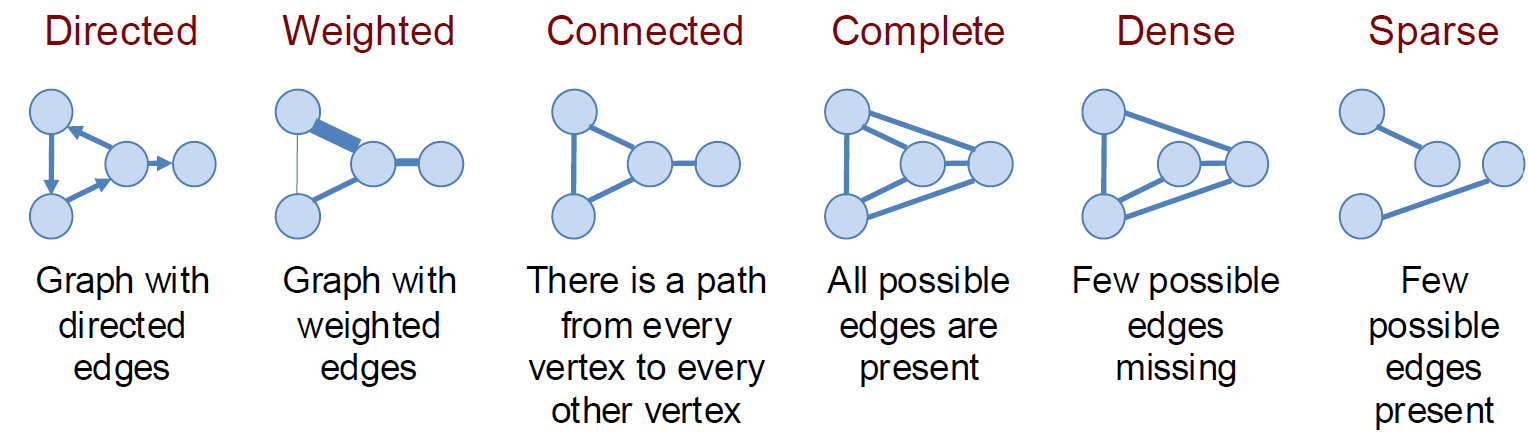
\includegraphics[width=0.85\textwidth]{img/graphs/DifferentGraphs.png}\end{center}
    \item \textbf{Valence of degree of vertex:} Number of edges a vertex lies on (in context of molecules: valence)
    \item \textbf{Adjacent vertices:} Vertices connected by an edge (in context of molecules: neibouring atoms)
    \item \textbf{Path:} List of distinct vertices in which successive vertices are connected by edges
    \begin{itemize}
        \item Simple Path: path with no vertex occurring twice
        \item Cycle Path: simple path of which first and last vertex are the same
    \end{itemize}
    \begin{center}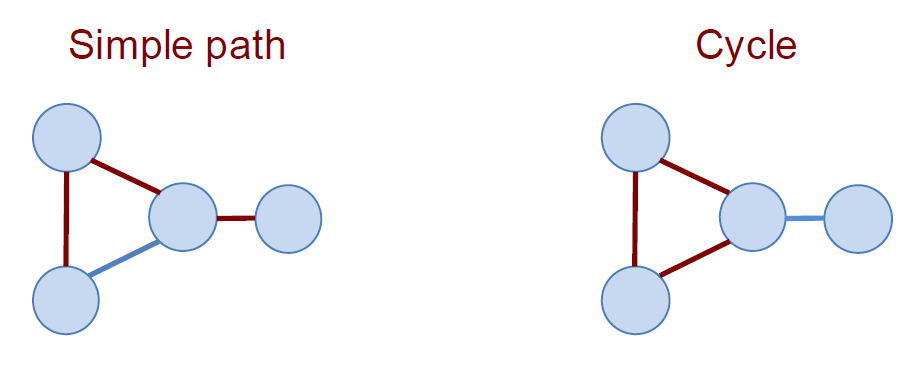
\includegraphics[width=0.85\textwidth]{img/graphs/PathGraphs.png}\end{center}
    \item \textbf{Trees:} (in graph theory)
    \begin{itemize}
        \item \textbf{Tree:} non-empty, acyclic collection of nodes and edges (graph) in which any 2 nodes are connecteds by exactly 1 path.  
        \item \textbf{Ordered Tree:} tree with order in the children nodes
        \item \textbf{Binary Tree:} ordered tree in which each non-terminal node has exactly two children
        \item \textbf{Binary Search Tree:} ordered binary tree with left-to-right order
        \item \textbf{Heap:} ordered binary tree with top-to-bottom order
    \end{itemize}
    \begin{center}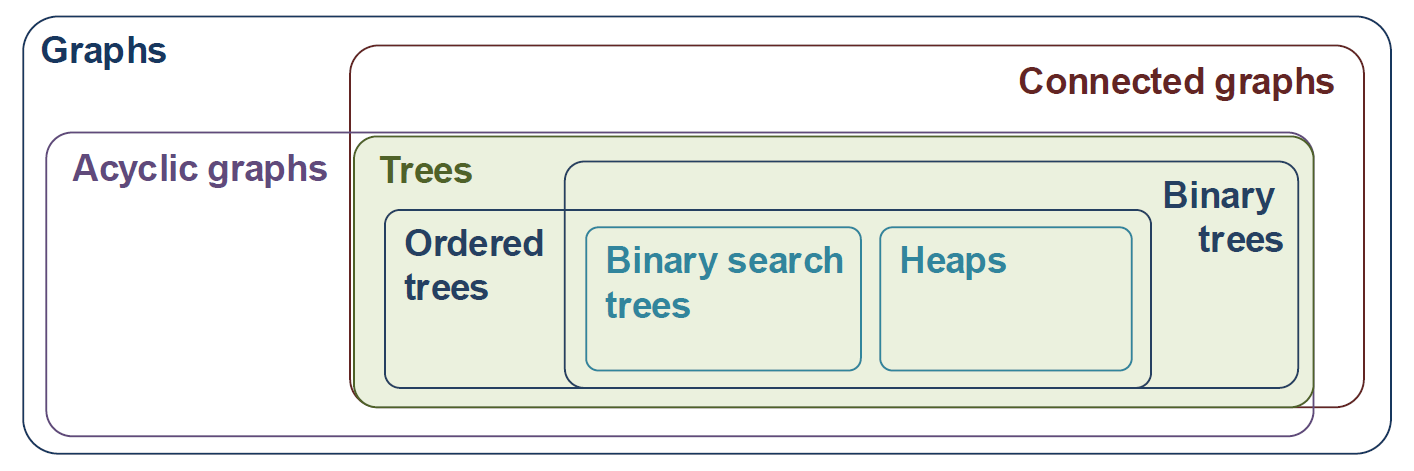
\includegraphics[width=0.85\textwidth]{img/graphs/GraphsTrees.png}\end{center}
\end{itemize}

\subsection{Representations of graphs}

A graph $G(V,E)$ with vertices $V$ and edges $E$ can be represented as a adjacency matrix (good for dense graphs) or an adjacency list (good for sparse graphs). 

\begin{center}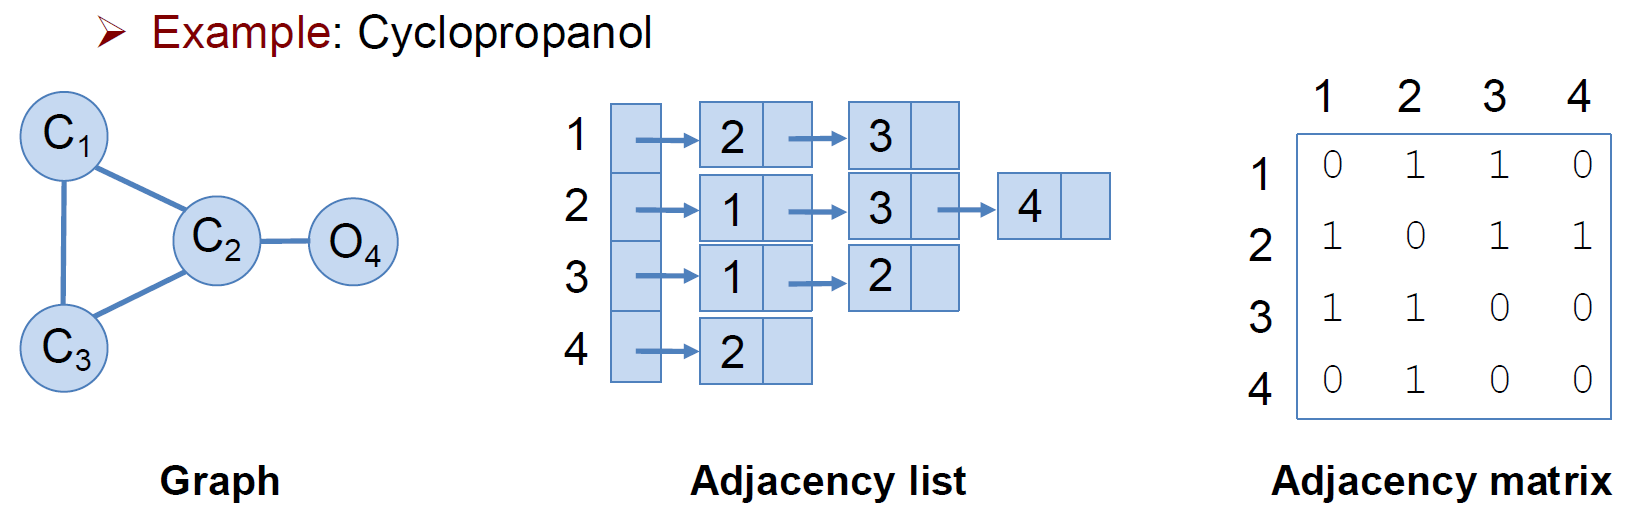
\includegraphics[width=0.85\textwidth]{img/graphs/MatrixVsList.png}\end{center}

\begin{table}[H]
    \centering
    \begin{tabular}{p{30mm} | p{50mm} | p{50mm}}
        \toprule
        \textbf{Function} & \textbf{Adjacency list} & \textbf{Adjacency matrix} \\
        \midrule
        \lstinline|size()| & Easy, size of a vector & Easy, soize of a vector \\
        \midrule
        \lstinline|isConnected()| & Difficult, search in linked list & Easy, direct access \\
        \midrule
        \lstinline|getNeighbours()| & Easy, copy of linked list & Difficult, search in row \\
        \midrule
        \lstinline|addEdge()| & Easy, append linked list & Easy, set matrix element to 1 \\
        \bottomrule
    \end{tabular}
\end{table}

\subsubsection{Adjacency list}

%\lstinputlisting[language=C++]{src/graphs/graph_list.cpp}

\subsubsection{Adjacecy matrix}

%\lstinputlisting[language=C++]{src/graphs/graph_matrix.cpp}

\subsection{Searching a graph}

When searching for a vertex in a graph, two different algorithms can be used: the first depth-first, the second breadth-first.

\subsubsection{Breadth-first (BF) search}

The breadth-first algorithm starts with a specific source vertex $s$, from which all vertices that can be reached from $s$ are discovered. This creates a breadth-first tree with the root $s$ and all reachable vertices.  During the algorithm, the shortest path (distance) from $s$ to $v$ is also determined for each vertex $v$. The vertices have three possible states:

\begin{itemize}
    \item \textbf{white:} undiscovered
    \item \textbf{gray:} discovered but with undiscovered neighbours
    \item \textbf{black:} discovered and all neighbours are discovered as well
\end{itemize}

All gray vertices are in a queue so that they can be processed one after the other. The running time of the algorithm is $\Theta(V+E)$.

Procedure:
\begin{enumerate}
    \item First, only the given root $s$ is gray.
    \item All neighboring vertices of $s$ become gray, their distance is 1 and $s$ becomes black.
    \item All neighbors of the gray vertices become gray, their distance is 2 and the former gray vertices become black. The gray vertices in the queue are processed one after the other.
\end{enumerate}

\begin{center}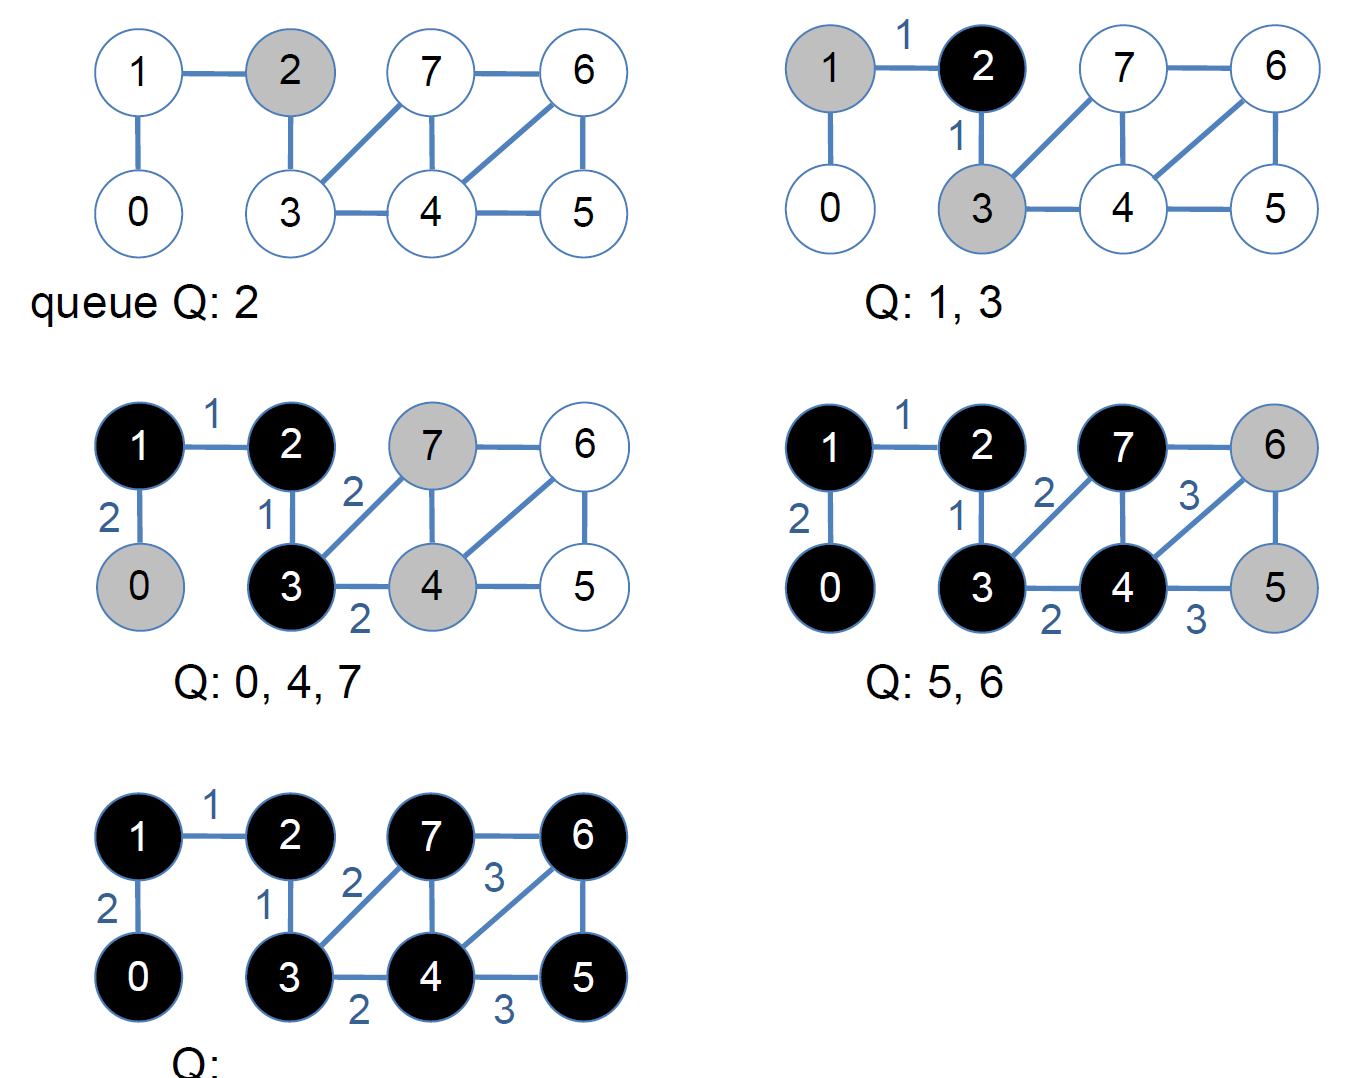
\includegraphics[width=0.85\textwidth]{img/graphs/BfSearch.png}\end{center}

% finished code, but without outpur of the searching
%\lstinputlisting[language=C++]{src/graphs/bf_search.cpp}

\subsubsection{Depth-first (DF) search}

If possible, the depth-first algorithm always searches deeper in the tree first and not as broadly as possible as with the BF algorithm. This creates a depth-first forest. Here, too, you start with a source vertex $s$ and discover all vertices that can be reached via $s$, but the three classifications of the vertices are slightly different:

\begin{itemize}
    \item \textbf{white:} undiscovered
    \item \textbf{gray:} first discovered (time $d$)
    \item \textbf{black:} all neighbours are discovered (time $f$)
\end{itemize}

The running time of the algorithm is $\Theta(V+E)$. If vertices remain after the algorithm that cannot be reached from the source $s$, the algorithm is continued via a new source $s$.

Procedure:
\begin{enumerate}
    \item First, only the given root $s$ is gray. (0)
    \item Then the neighbor of $s$ becomes gray with the smallest value. (1)
    \item Then the neighbor of (1) with the smallest value is grayed out again. (2) This continues until a vertex is found that has no neighbors. (3)
    \item Now the backtracking begins until a vertex is found that still has unexplored neighbors. This then turn gray and the procedure continues.
\end{enumerate}

% finished code, but without outpur of the searching
%\lstinputlisting[language=C++]{src/graphs/df_search.cpp}

\subsection{Minimum spanning trees}

The \emph{minimum spanning trees problem} is to turn a graph into a tree such that all vertices are connected and the sum of the edge weights is minimal. An important property of this tree is that if the vertices of the graph are arbitrarily divided into two sets, the minimum spanning tree always contains the shortest path between two vertices from both sets. In principle, two algorithms can be applied to the problem, namely \emph{Kruskal's algorithm} (good for sparse graphs) and \emph{Prim's algorithm} (good for dense graphs), which both run in $\Theta(E\lg V)$ time for a graph $G(V,E)$ with vertices $V$ and edges $E$.

\begin{center}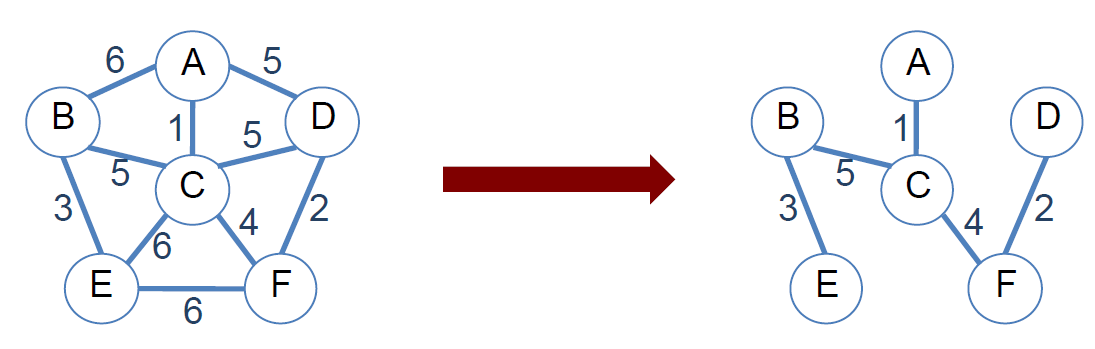
\includegraphics[width=0.85\textwidth]{img/graphs/MinimumSpanningTree.png}\end{center}

\subsubsection{Kruskal's algorithm}

In Kruskal's algorithm, the minimum spanning tree is constructed by joining a set of unconnected vertices together. The tree is therefore built from the root and no edges are deleted, which is why it is particularly suitable for sparse graphs.

Procedure:
\begin{enumerate}
    \item Put the edge with the lowest weight in a tree of the forest
    \item Put the edge into the forest with the next higher weight (algorithm follows ascending weights), provided that adding it does not create a cycle. If it does, skip that edge.
    \item Stop after $V-1$ edges have been considered (ensures that all vertices are connected to each other). 
\end{enumerate}

\begin{center}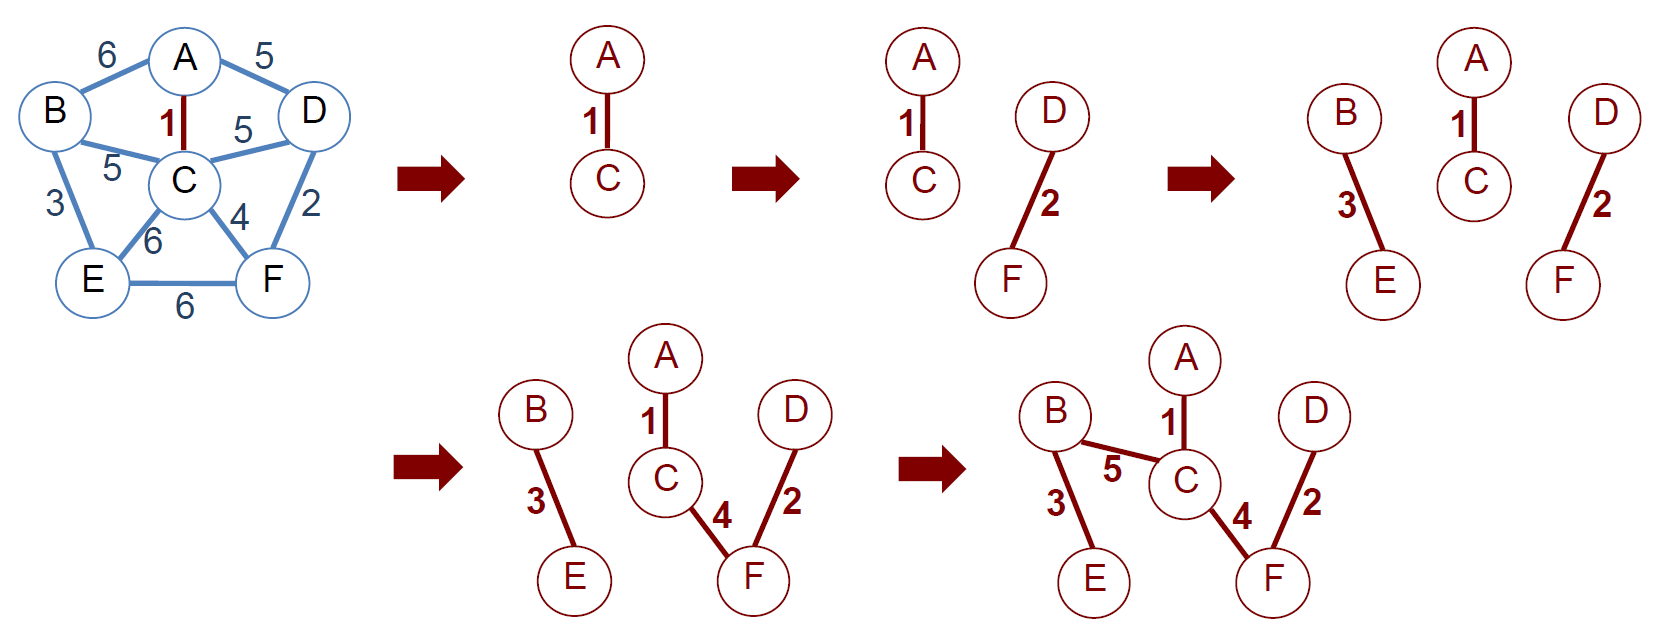
\includegraphics[width=0.85\textwidth]{img/graphs/KruskalGraph.png}\end{center}

%\lstinputlisting[language=C++]{src/graphs/kruskal.cpp}

\subsubsection{Prim's algorithm}

Prim's algorithm is a greedy algorithm.

Procedure:
\begin{enumerate}
    \item Put one random vertex on the tree (e.g. A)
    \item Find the edge with the lowest weight that connects A to a vertex, that is not in the tree yet. (C)
    \item Find from C the edge with the lowest weight that connects C to a vertex, that is not in the tree yet, but without building a cycle. (F)
    \item Continue finding edges with the lowest weight from the last vertex without building a cycle. If there is no edge to a vertex, without building a cycle, go back until you have a vertex with new neighbours.
    \item Stop if tree contains $V$ vertices or if no more edges can be found.
\end{enumerate}

\begin{center}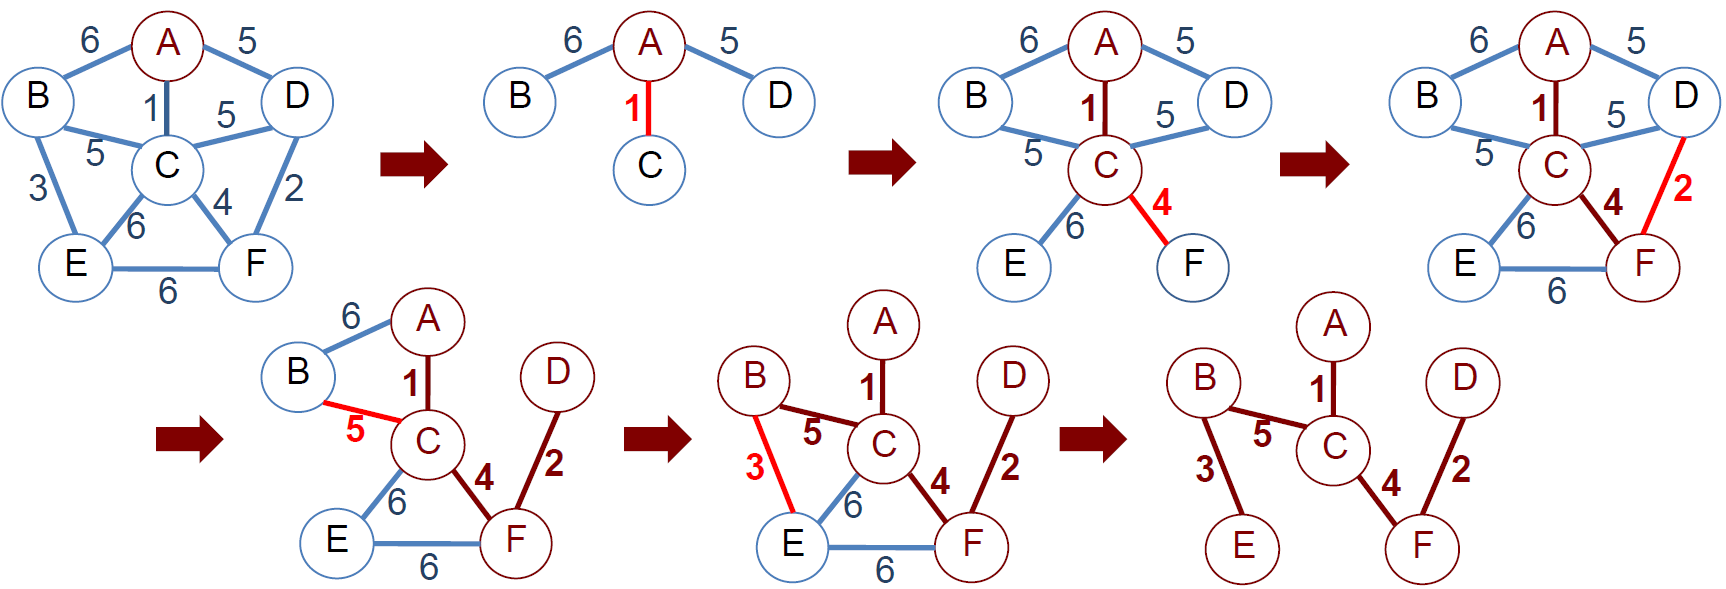
\includegraphics[width=0.85\textwidth]{img/graphs/PrimGraph.png}\end{center}

%\lstinputlisting[language=C++]{src/graphs/prim.cpp}

\subsection{Single-source shortest paths}

The \emph{Single-source shortest paths} is to determine the length $d_i$ of the shortest path from the source vertex $v_0$ (single source) to every other vertex $v_i$. For that we use an directed and weighted graph (only positive weights and directed edges) and the length $d_i$ of the path is the sum of the weights along its edges. One can use in principle two algorithms for that:

\begin{itemize}
    \item \textbf{Brute-force:} Try all combinations of edges with $\Theta((V-1)!)$
    \item \textbf{Dijkstra's algorithm} Greedy algorithm with $\Theta(V^2)$
\end{itemize}

\subsubsection{Dijkstra's algorithm}

Dijkkstra's algorithm is a greedy algorithm that can find the weight or distance $d_i$ of the shortest path from a given source vertex 
$v_0$ to each other vertex $v_i$ of the graph. It runs in a running time of $\Theta(V^2)$, which can be improved to $\Theta((V+E)\lg V)$ for a sparse graph and to $\Theta(E\lg V)$ for a sparse graph in which all vertices can be reached from the source vertex. To do this, the algorithm defines two sets of vertices:

\begin{itemize}
    \item Vertices that were already considered: Their shortest path is known.
    \item Vertices that have not been considered yet. 
\end{itemize}

During the algorithm, a distance table, which is initially the adjacency matrix of the graph, is continuously updated. The weights of the paths from all vertices to the source vertex are stored in a vector.

\begin{enumerate}
    \item First, determine the direct distance $d_i$ from the source vertex $v_0$ to each vertex $v_i$ of the graph ($d_i=\mathrm{weight}(v_0,v_i)$) and insert the distances into the path vector.
    \item Create a vector of the size of all vertices, which is initially set to zero for all elements. If a vertex has been taken into account, the vector element for this vertex becomes one. 
    \item Make a loop over all vertices (An index k is defined which maps to the vertex currently being considered, but which is not the loop index. At the beginning: $k=v_0$):
    \begin{enumerate}
        \item Identify the vertex that is at the smallest distance from the source vertex $v_0$ and was not considered yet (the distances of the path vector are used). This vertex has now been taken into account, is now the current vertex and is set to one in the consideration vector.
        \item Go over all vertices that have not yet been considered and check whether the shortest path to the current vertex $v_k$ plus the distance to the new vertex is smaller than the distance stored in the path vector. If yes. update the path vector.
    \end{enumerate}
\end{enumerate}

\begin{center}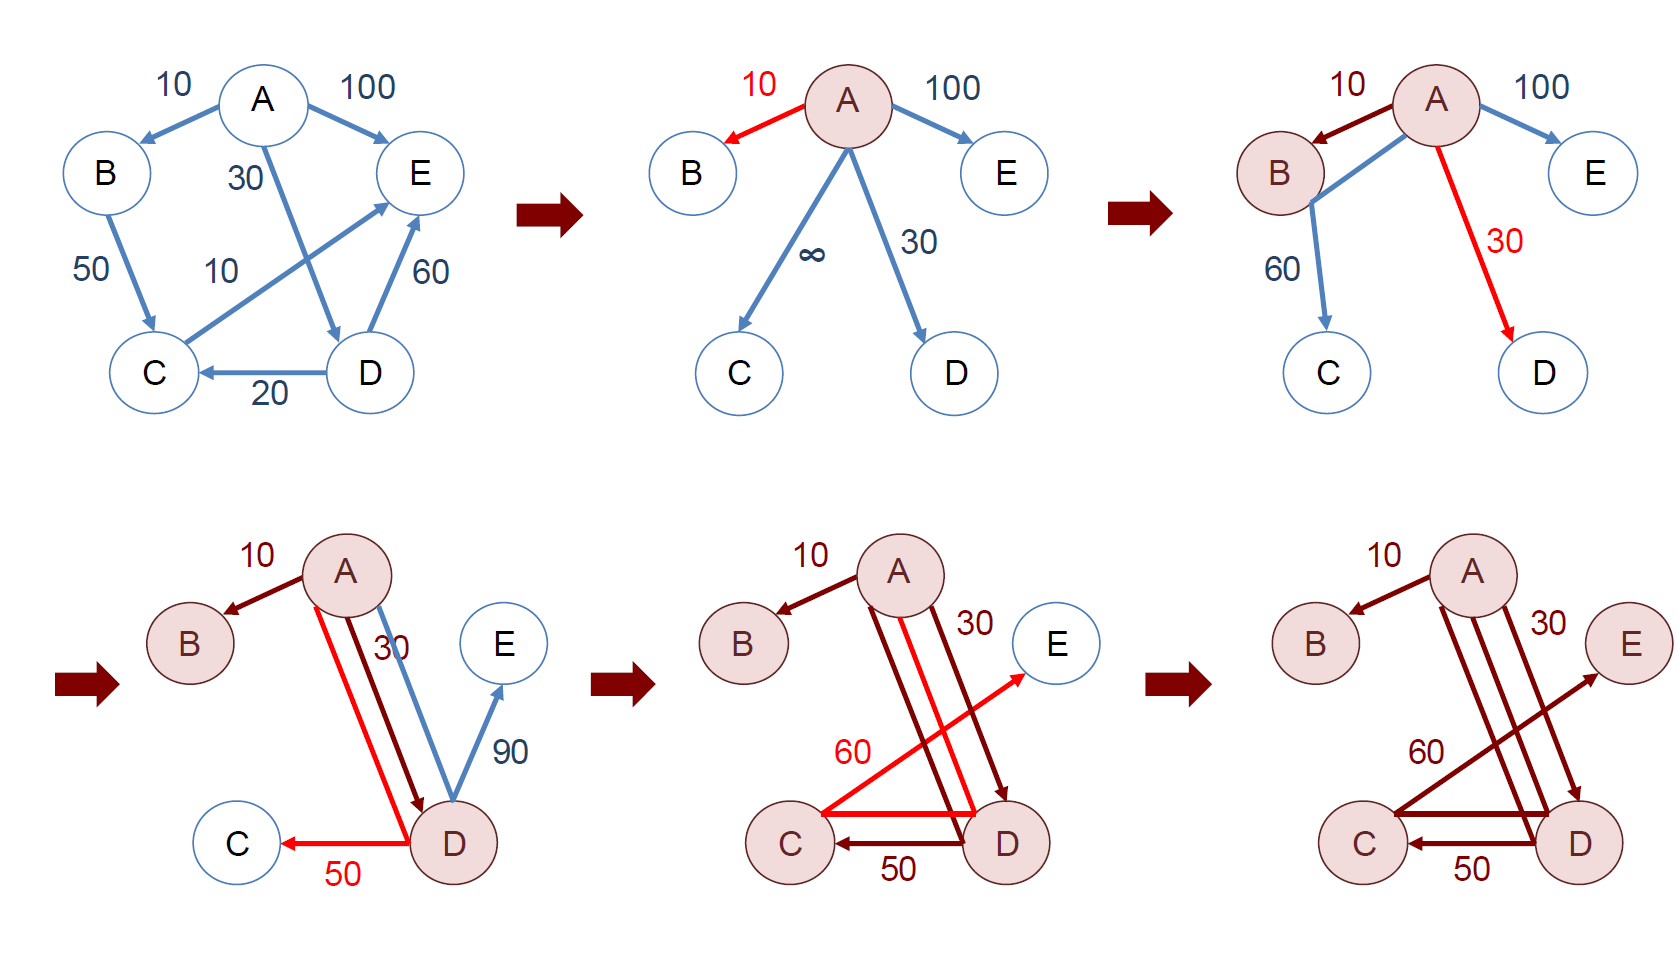
\includegraphics[width=0.85\textwidth]{img/graphs/DijkstraGraph.png}\end{center}

\begin{center}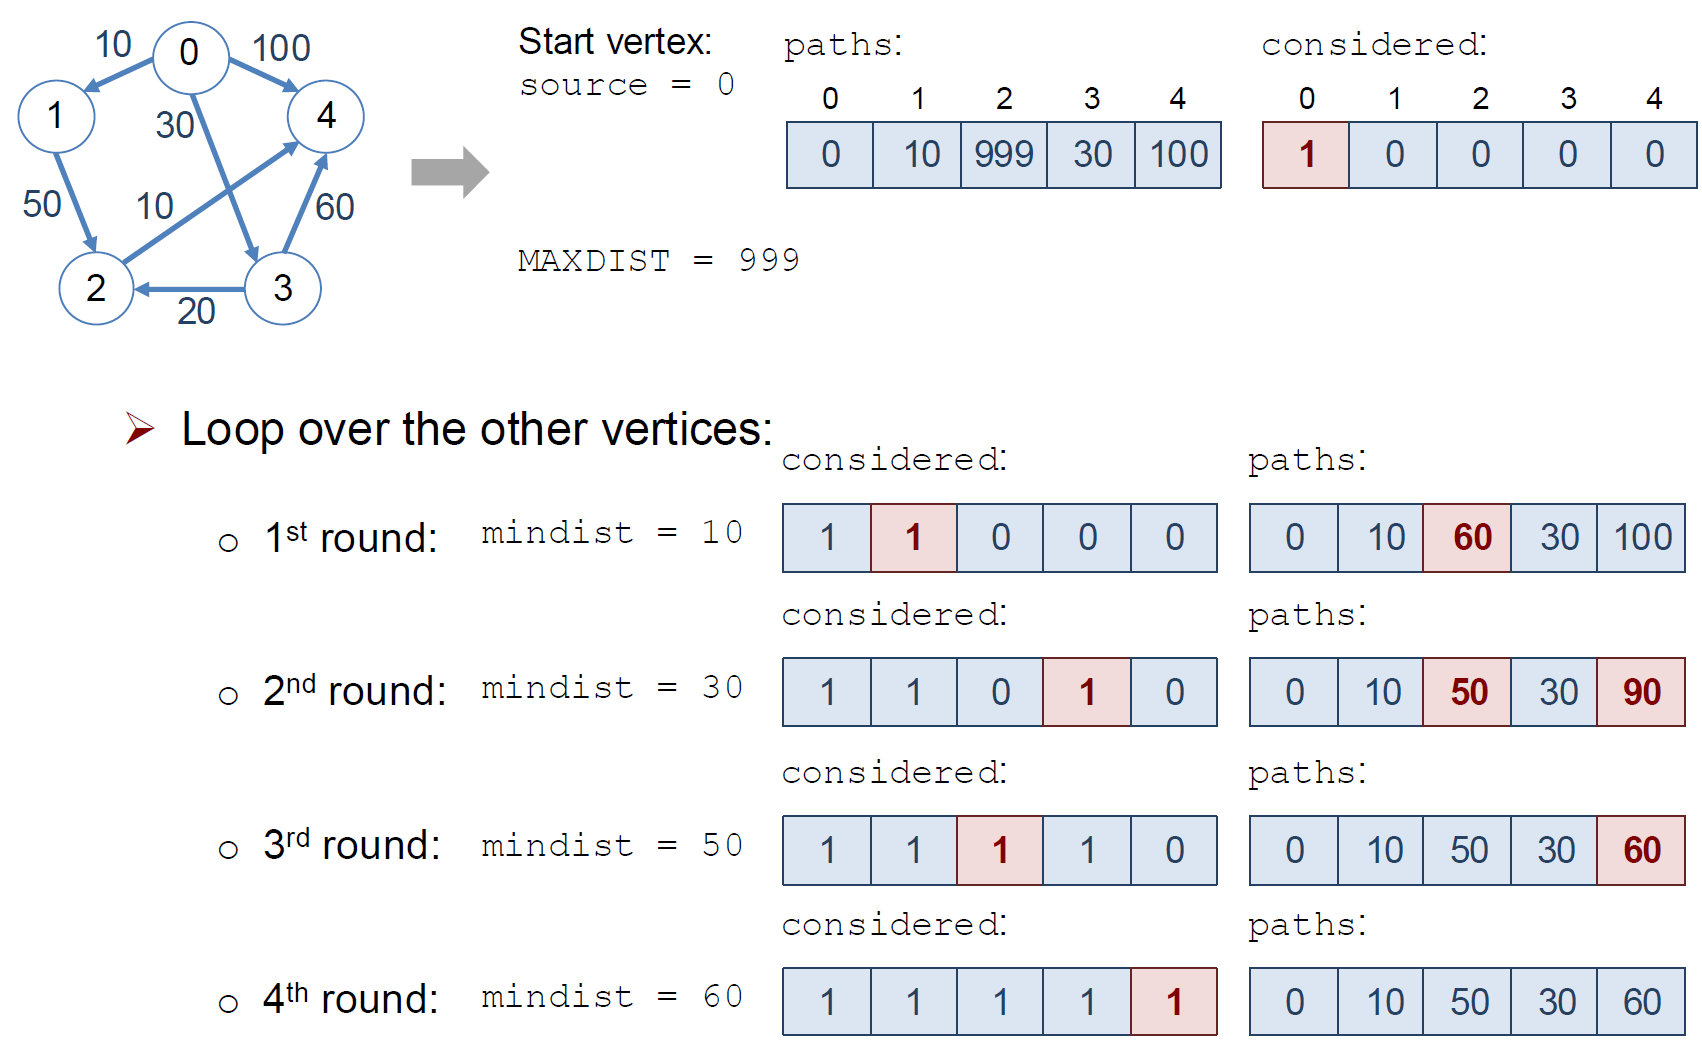
\includegraphics[width=0.85\textwidth]{img/graphs/DijkstraVectorGraph.png}\end{center}

%algorithmus ist fertig
%\lstinputlisting[language=C++]{src/graphs/dijkstra.cpp}

\subsection{All-pair shortest paths}

The \emph{All-pair shortest paths} problem is to do the single-source shortest paths problem on every vertex of a graph so that you get the length $d_{ij}$ of the shortest path between every two vertices of the graph. Here negative weights of the edges are also possible. For this problem you can choose between two algorithms.

\begin{itemize}
    \item \textbf{Dijkstra's algorithm starting at each vertex}
    \begin{itemize}
        \item Only if weights are all positive
        \item Running time: $\Theta(V^3)$ (With improvements: $\Theta(V(V+E)\lg V)$ or $\Theta(VE\lg V)$)
        \item Good for sparse graphs
    \end{itemize}
    \item \textbf{Floyd-Warshall algorithm}
    \begin{itemize}
        \item Running time: $\Theta(V^3)$
        \item Good for dense graphs
    \end{itemize}
\end{itemize}

\subsubsection{Floyd-Warshall algorithm}

The Floyed-Warshall algorithm is a \emph{dynamic programming} algorithm to determine the shortest path between each vertex of a graph and, unlike the Dijkstra's algorithm, can also handle negative edge weights. The running time is $\Theta(V^3)$, but the inner loop is very simple. The idea of the algorithm is to compare all possible paths in the graph and to build an increasingly better distance matrix to determine the shortest paths. To do this, it checks for each vertex whether it is better to take the direct route from $v_i$ to $v_j$ or to include the vertex $v_k$ as an intermediate step.

\begin{enumerate}
    \item Loop over all vertices $k$
    \item Check for each pair of vertices $v_i$ and $v_j$ whether the distance $d_{ij}$ can be made shorter via vertex $v_k$
    \begin{itemize}
        \item \lstinline|shortestPath(i,j,k)| returns the shortest possible path from $v_i$ to $v_j$ using only vertices from the set $\{1,2,\cdots,k\}$
    \end{itemize}
\end{enumerate}

\begin{center}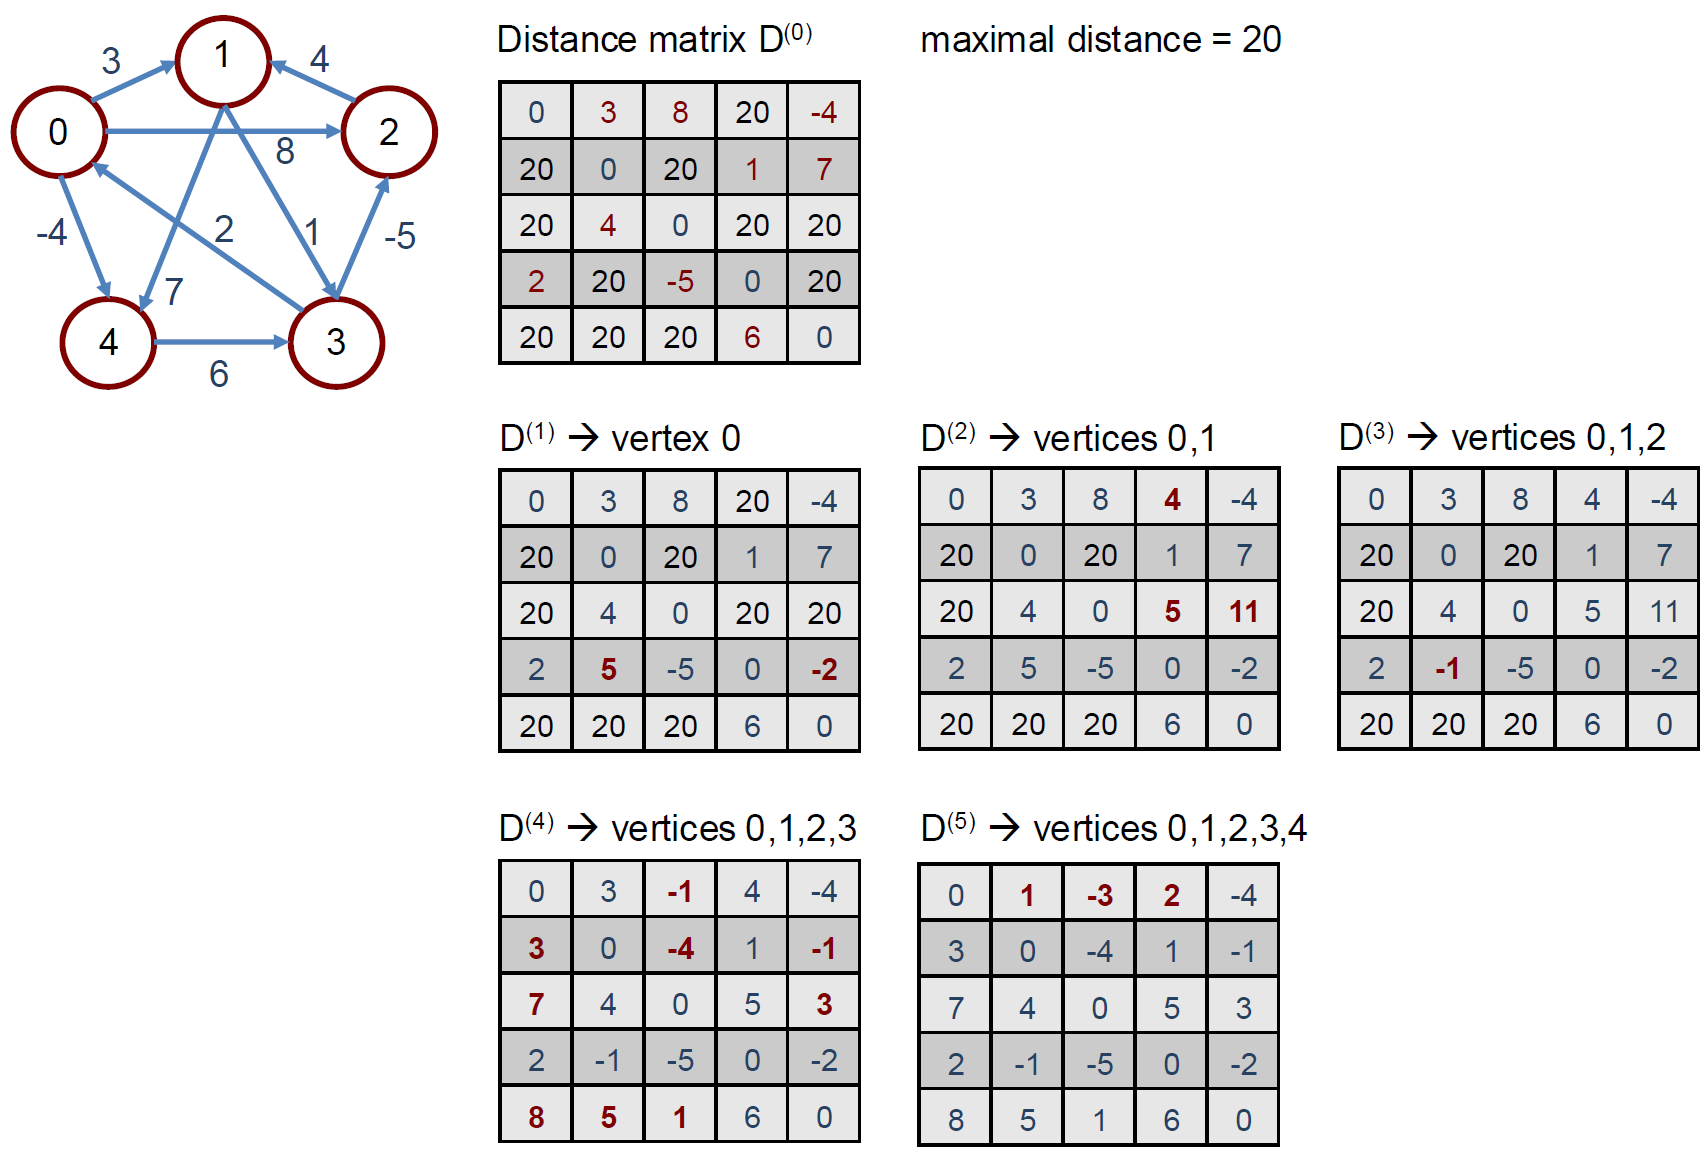
\includegraphics[width=0.85\textwidth]{img/graphs/FloydWarshallGraph.png}\end{center}

%algorithmus ist fertig
%\lstinputlisting[language=C++]{src/graphs/floyed_warshall.cpp}

% tex: Ca. Hälfte
% src: mehr als hälfte
\newpage\section{Approximation Algorithms}% Approximation Algorithms (1 week)

Often, it is not necessary to find the best solution to a problem, but an approximation of the best solution (i.e. a good solution) is sufficient. In addition, the algorithms for the exact solution are usually very complex and the running time plays a central role in the evaluation of an algorithm.

\begin{itemize}
    \item \textbf{Turing machine}
    \begin{itemize}
        \item To compare the complexity or difficulty of an algorithm, we need to define a model computer on which the algorithm is to run.
        \item \emph{Deterministic Turing machine:} Processes an algorithm a step at a time (normal computer)
        \item \emph{Non-Deterministic Turing machine:} Can do multiple steps at a time (fictitious computer)
    \end{itemize}
    \item \textbf{Complexity classes}
    \begin{itemize}
        \item \emph{P:} Set of decision problems that can be solved by a deterministic Turing machine in \textbf{p}olynomial time
        \item \emph{NP:} Set of decision problems that can be solved by a \textbf{n}on-deterministic Turing machine in \textbf{p}olynomial time
        \item All problems in \textbf{P} are also in \textbf{NP} (Open question: Are all problems in \textbf{NP} also in \textbf{P})
    \end{itemize}
    \item \textbf{Problem reduction}
    \begin{itemize}
        \item \emph{Reducibility:} Problem $X$ can be transformed into problem $Y$ by a reduction function such that the answers of $X$ and $Y$ are the same.
        \item If a problem $X$ can be reduced to problem $Y$, each algorithm solving $Y$ can also be used to solve $X$ (If there is a polynomial-time algorithm for problem $Y$, there is also one for $X$).
        \item e.g. Problem of taking the square of a number is polynomial-reducible to the problem of multiplying two numbers.
    \end{itemize}
    \item \textbf{NP-completeness}
    \begin{itemize}
        \item 
    \end{itemize}
\end{itemize}

Most of the problems that we want to solve with approximation algorithms are NP-complete, which is because they follow a boolean logic, are subject to the graph data type, etc. When designing an algorithm, the main goal is to find the optimal solution quickly for all possible cases. Since this is virtually impossible for an approximation, we follow these steps:

\begin{itemize}
    \item Relax requirement for \emph{speed:} If N is small, an algorithm with exponential running time might be okay.
    \item Relax requirement for \emph{generality:} Isolate important special cases that can be solved in polynomial time.
    \item Relax requirement for \emph{optimal solution:} Find near-optimal solutions (approximations) in polynomial time (either worst-case or average case) à in practice, this is often good enough
\end{itemize}

A well-known problem from the world of approximation algorithms is the \emph{Traveling Salesman Problem} (TSP), in which the optimal path in a graph (undirected, weighted dense graph) is to be found, in which each vertex is visited exactly once and one starts at the same vertex as one ends. 

\begin{center}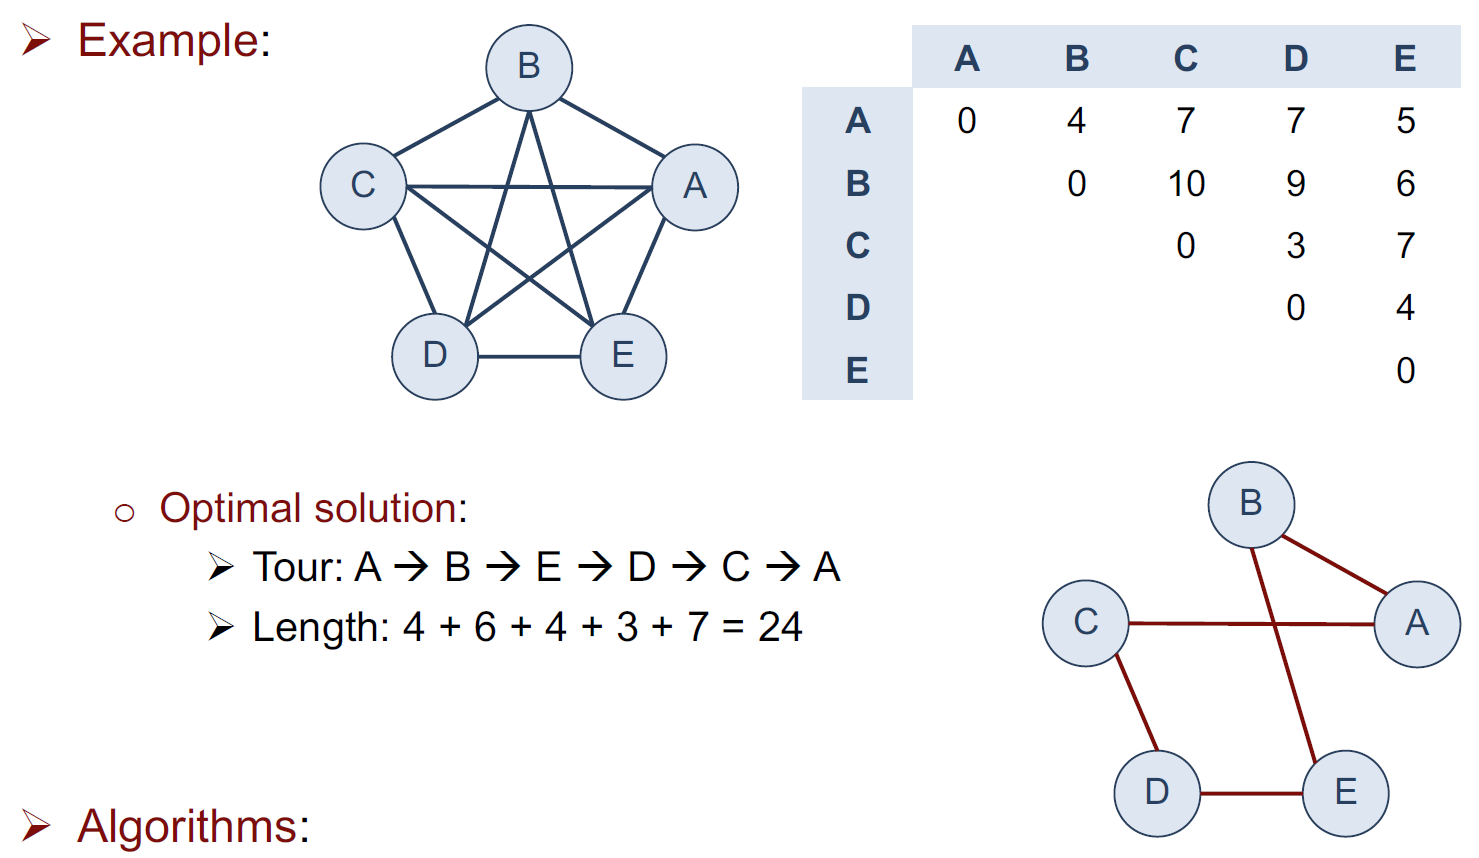
\includegraphics[width=0.85\textwidth]{img/approximation/TspOptimalSolution.png}\end{center}

It is a NP-hard optimization problem and worst-case running time is superpolynomial with $\Theta(N!)$. There are four broad types of approximation algorithms:

\begin{itemize}
    \item \textbf{Greedy Algorithm}
    \begin{itemize}
        \item At each decision point, select the option that yields the largest immediate progress towards the goal.
        \item Running time for TSP: $\Theta(N)$
    \end{itemize}
    \item \textbf{Local search}
    \begin{itemize}
        \item Guess an arbitrary solution and try to improve.
        \item Running time for TSP: difficult to estimate, but usually very efficient
    \end{itemize}
    \item \textbf{Approximate dynamic programming}
    \begin{itemize}
        \item Combine the solutions of subproblems.
        \item Running time for TSP: $\Theta(N^22^N)$
    \end{itemize}
    \item \textbf{Backtracking with heuristics}
    \begin{itemize}
        \item 
        \item Running time for TSP: difficult to estimate
    \end{itemize}
\end{itemize}

\subsection{Approximate dynamic programming}

The idea of the dynamic programming approach is to first solve subproblems of the actual problem and then combine them to find a solution. To do this, we define $S$ as the set of vertices that have not yet been visited. We start the journey at 0 and the journey ends at vertex $j\in\{1,2,\cdots,N-1\}$, where $N$ is the number of vertices. We denote the problem as $C(S,j)$ (mathematically, $C(S,j)$ is the total cost of the path), where the journey starts at 0, ends at $j$ and in between all vertices of the set $S$ without $j$ are visited. So the subproblem is to find the minimum for a vertex $i$ (penultimate vertex) that is in $S$ and is not $j$, so that we have reduced the overall problem by one vertex to $C(S-\{i\},i)$ and can raise it back to the overall problem by adding the distance $d_{i,j}$.

\begin{align}
    C(S,j)=\min_{i\in S\;i\neq j}\left\{d_{i,j}+C(S-\{i\},i)\right\}
\end{align}

Thus, we generate $N^22^N$ subproblems, each of which has a linear running time, which is why overall we have a running time of $\Theta(N^22^N)$. We want to stay at the example above We proceed as follows to implement the algorithm:

\begin{enumerate}
    \item $C(\{\},j)$ is the shortest path from $0$ to $j$, but all cities besides $j$ was already visited, so $C(\{\},j)=d_{0,j}$ is the only possible path.
    \item We first calculate all possible combinations of $C(\{S\},j)$, where only one city was not visited yet, so that $|S|=1$. Because this is a problem of we start from 0, end up $j$ and we have to visit only one city in between that, there is only one possible path for this, so we do not have to calculate an minimum.
    \begin{align*}
        C(\{1\},2)&=d_{1,2}+C(\{\},1)=d_{1,2}+d_{0,1}=14\\
        C(\{2\},1)&=d_{2,1}+C(\{\},2)=d_{2,1}+d_{0,2}=17\\
        C(\{1\},3)&=d_{1,3}+C(\{\},1)=d_{1,3}+d_{0,1}=13\\
        C(\{3\},1)&=d_{3,1}+C(\{\},3)=d_{3,1}+d_{0,3}=16\\
        C(\{1\},4)&=d_{1,4}+C(\{\},1)=d_{1,4}+d_{0,1}=10\\
        C(\{4\},1)&=d_{4,1}+C(\{\},4)=d_{4,1}+d_{0,4}=10\\
        C(\{2\},3)&=d_{2,3}+C(\{\},2)=d_{2,3}+d_{0,2}=10\\
        C(\{3\},2)&=d_{3,2}+C(\{\},3)=d_{3,2}+d_{0,3}=11\\
        C(\{2\},4)&=d_{2,4}+C(\{\},2)=d_{2,4}+d_{0,2}=14\\
        C(\{4\},2)&=d_{4,2}+C(\{\},4)=d_{4,2}+d_{0,4}=12\\
        C(\{3\},4)&=d_{3,4}+C(\{\},3)=d_{3,4}+d_{0,3}=11\\
        C(\{4\},3)&=d_{4,3}+C(\{\},4)=d_{4,3}+d_{0,4}=9
    \end{align*}
    \item Now we can increase the size of $S$ by one, so that we have $|S|=2$, but with that we have two possible values for $i$. Because of that we now have to determine a minimum between two values, but when we use the formula to reduce the problem to a smaller size of $S$, we can use the values above.
    \begin{align*}
        C(\{1,2\},3)&=\min_{i\in\{1,2\}}\left\{d_{i,3}+C(\{1,2\}-\{i\},i)\right\}\\
        &=\min\left\{\{d_{1,3}+C(\{2\},1)\},\{d_{2,3}+C(\{1\},2)\}\right\}\\
        &=\min\left\{\{9+17\},\{3+14\}\right\}=\min\{28,17\}=17\\
    \end{align*}
    \item We continue to increase the size of $S$ by one until we get to our final $S$ and fill in each step the values from before to determine the min. 
    \begin{align*}
        C(\{1,2,3\},4)&=\min_{i\in\{1,2,3\}}\left\{d_{i,4}+C(\{1,2,3\}-\{i\},i)\right\}\\
        C(\{1,2,3,4\},0)&=\min_{i\in\{1,2,3,4\}}\left\{d_{i,0}+C(\{1,2,3,4\}-\{i\},i)\right\}\\
    \end{align*}
\end{enumerate}

% finished code (but with out comments)
%\lstinputlisting[language=C++]{src/approximation/dynamic.cpp}

\subsection{Backtracking with heuristics}



% not finished code
%\lstinputlisting[language=C++]{src/approximation/backtracking.cpp}

\subsection{Greedy algorithm}

A greedy algorithm is based on always making the decision with the smallest weight from a starting point, so in terms of graph theory, that you start at a certain vertex and from there always select the edge with the smallest weight. At TSP, we proceed as follows, always keeping in mind that the result depends on the starting vertex:

\begin{enumerate}
    \item Start from a random city.
    \item Go to the nearest city not visited yet.
    \item Repeat until all cities have been visited and finally return to starting city.
\end{enumerate}

\begin{center}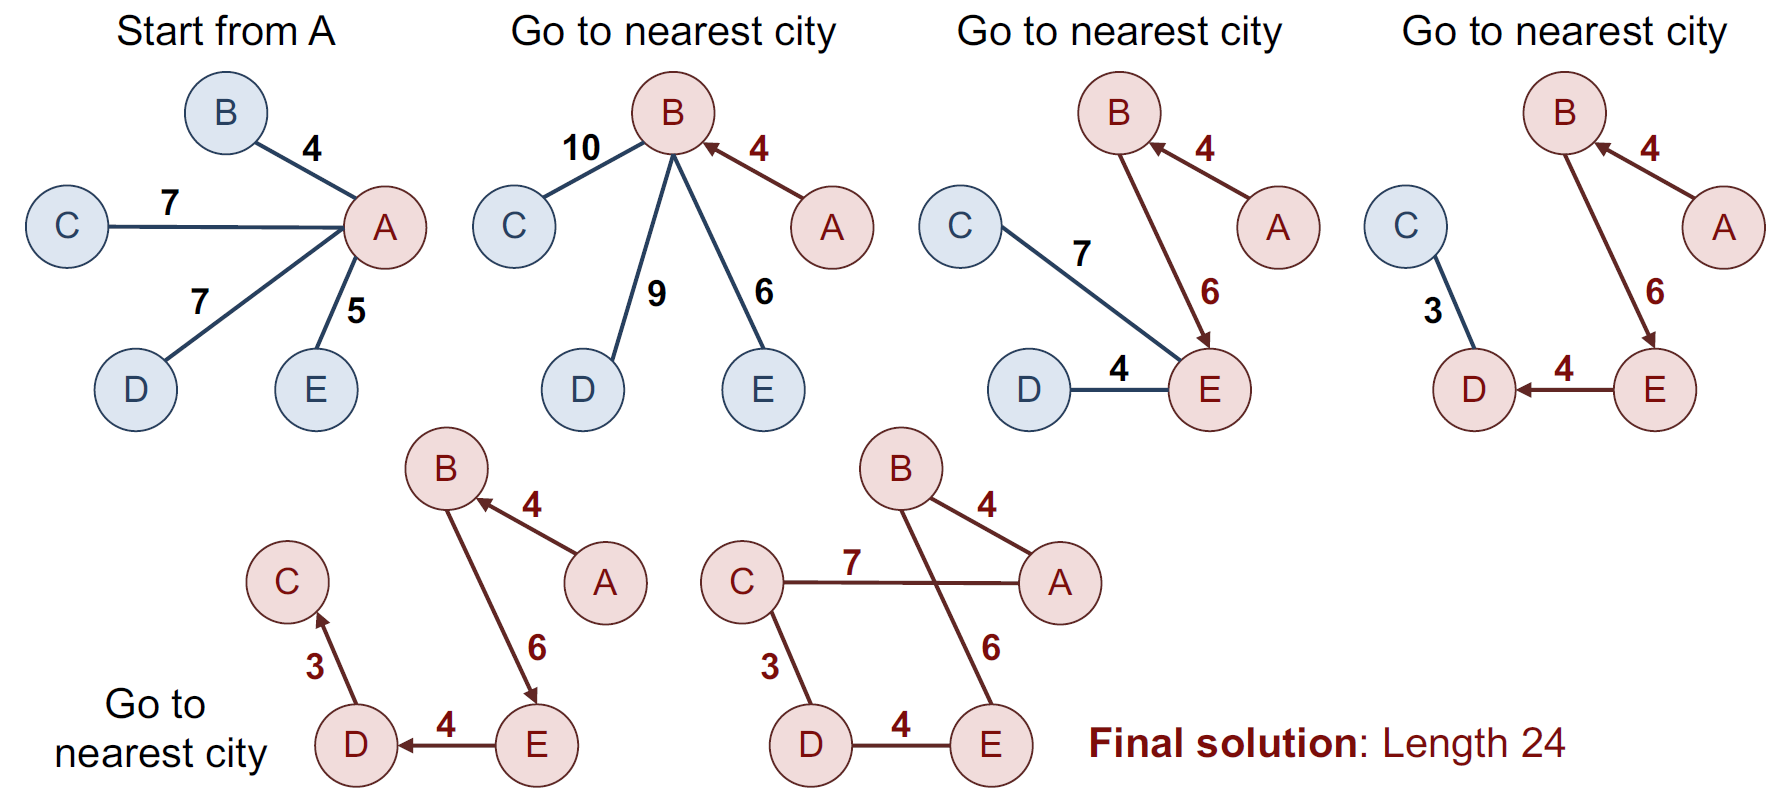
\includegraphics[width=0.85\textwidth]{img/approximation/TspGreedy1.png}\\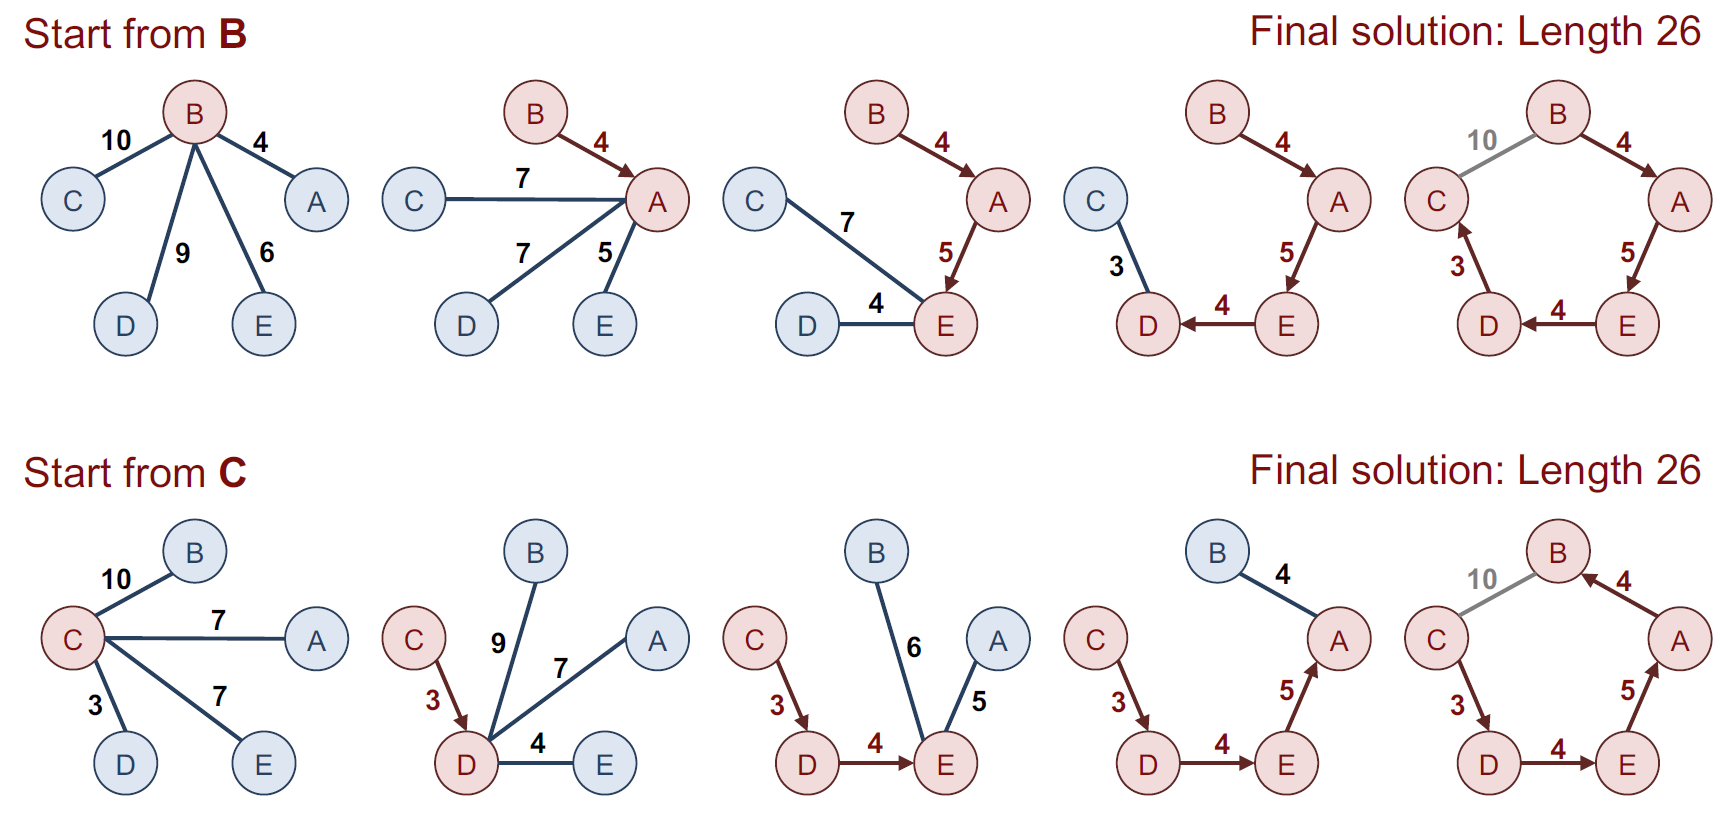
\includegraphics[width=0.85\textwidth]{img/approximation/TspGreedy2.png}\\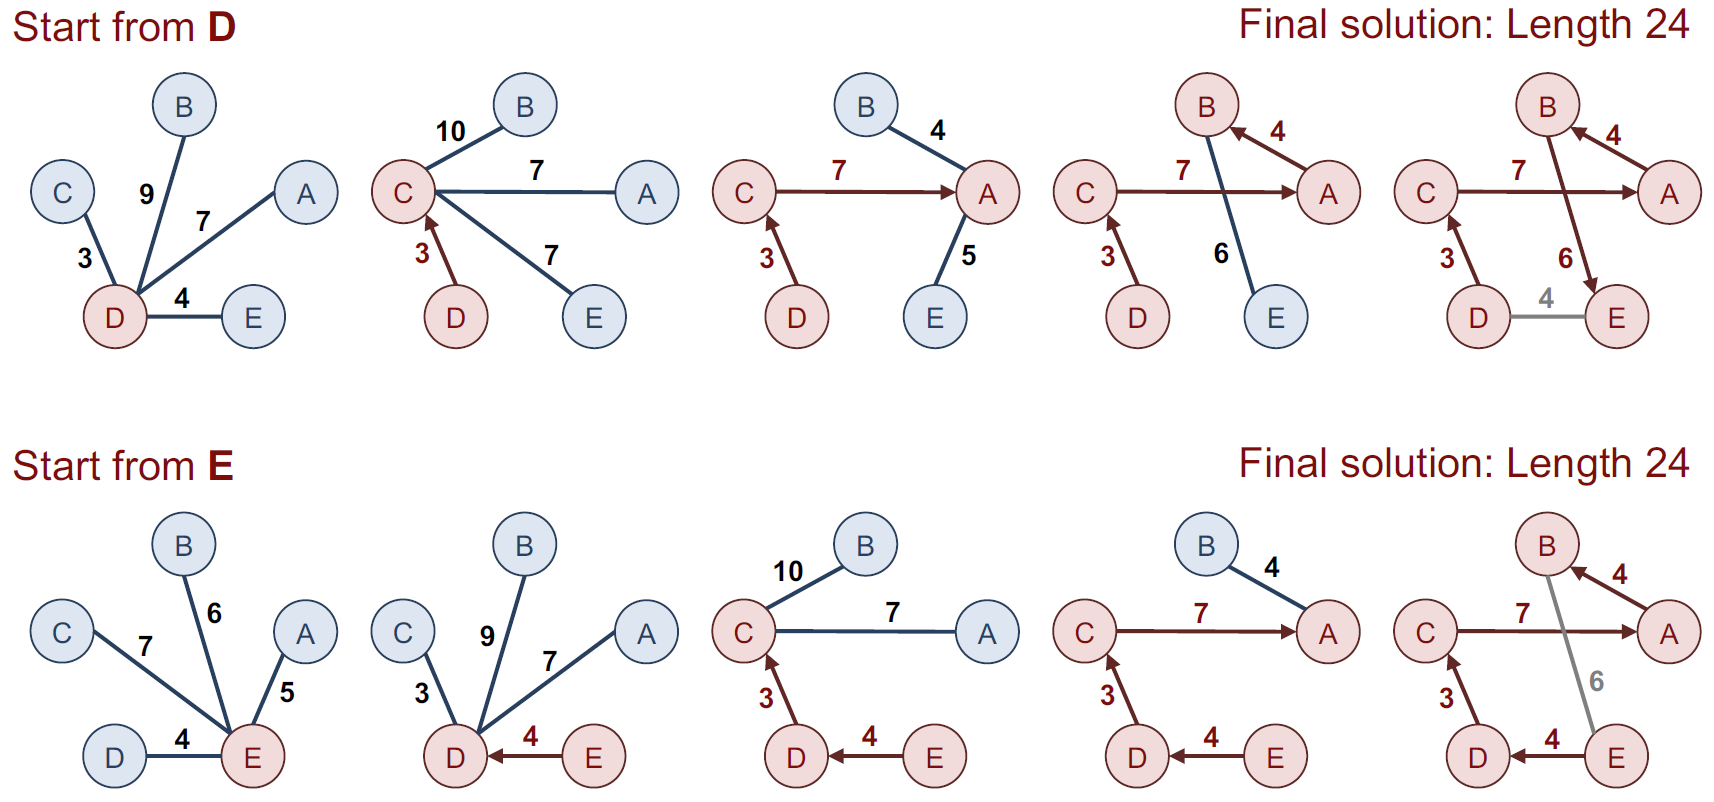
\includegraphics[width=0.85\textwidth]{img/approximation/TspGreedy3.png}\end{center}

% finished code
%\lstinputlisting[language=C++]{src/approximation/greedy.cpp}

\subsection{Local search}

The local search approach generally involves guessing a solution to the problem and then improving this solution by swapping. Applied to the TSP, this involves guessing a possible path and swapping two cities and calculating the length of the new path until the length can no longer be reduced. The central problem with the local search algorithm, however, is that it can get stuck at local minima of the problem, which can be somewhat improved with tweaks such as more complicated swapping. The algorithm proceeds as follows:

\begin{enumerate}
    \item Guess a solution.
    \item Interchange two cities and evaluate new tour $\rightarrow$ take if length decreases.
    \item Repeat this step until the length can no longer be reduced.
\end{enumerate}

\begin{center}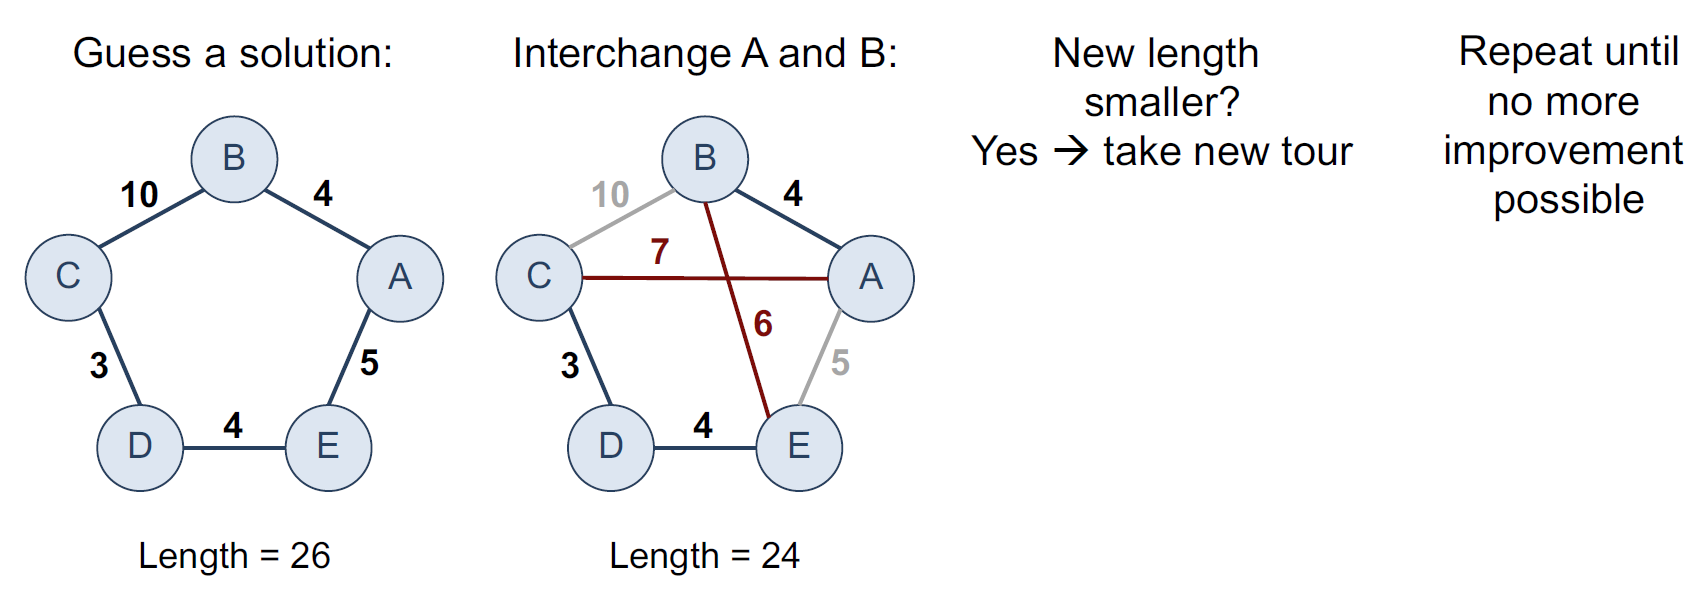
\includegraphics[width=0.85\textwidth]{img/approximation/TspLocalSearch.png}\end{center}

% not finished code
%\lstinputlisting[language=C++]{src/approximation/local_search.cpp}



% tex: 
% src: 
\newpage\section{Numerical Algorithms}\subsection{Systems of Equations}

\subsubsection{Gauss-elimination}

\textit{Given a Matrix of $\mathrm{N^2}$ dimensions, the Gauss-elimination algorithm will perform a classical gauss elimination as done on paper. For a given Matrix A, and its corresponding coefficient vector b, it will stepwise apply equation \ref{eq: Gauss_elim}. Keep in mind, that the actual algorithm will not have a separate b vector, but instead one largeer A matrix with N rows and N+1 columns}

\begin{align}
    A[j][k] = A[j][k] - A[i][k] \cdot \frac{A[j][i]}{A[i][i]}
    \label{eq: Gauss_elim}
\end{align}

\begin{align*}
    \begin{bmatrix}
        5 & 2 & 1 \\
        2 & 2 & 7 \\
        6 & 2 & 3 \\
    \end{bmatrix}
    =
    \begin{bmatrix}
        5 \\
        3 \\
        3 \\
    \end{bmatrix}
\end{align*}

\textit{The algorithm loops over all rows i and sets element A[j][k] to the new value. This is done by subtracting a[i][k] (so the value of the same column, one row above) with the adjusting factor $\mathrm{\frac{A[j][i]}{A[i][i]}}$, which is the first non-zero element of row j, divided by the first non-zero element of i, which is also the diagonal element. Note that k (the column iterator) starts at the right, as it would otherwise overwrite the first element of the j row, which would become zero, giving the false result for the other elements.}

\textit{For the $\mathrm{2^{nd}}$ row, the algorithm will apply equation \ref{eq: Gauss_elim} as follows}

\begin{align*}
    \begin{bmatrix}
        5 & 2 & 1 \\
        \color{red}2 & \color{red}2 & \color{red}7 \\
        6 & 2 & 3 \\
    \end{bmatrix}
    =
    \begin{bmatrix}
        5 \\
        \color{red}3 \\
        3 \\
    \end{bmatrix}
\end{align*}

\begin{align*}
    A[2][1] &= 2 - 5 \cdot \frac{2}{5} = 0 \\
    A[2][2] &= 2 - 2 \cdot \frac{2}{5} = 1.2 \\
    A[2][3] &= 7 - 1 \cdot \frac{2}{5} = 6.6 \\ \\
    b[2] &= 3 - 5 \cdot \frac{2}{5} = 1
\end{align*}

\begin{align*}
    \begin{bmatrix}
        5 & 2 & 1 \\
        \color{red}0 & \color{red}1.2 & \color{red}6.6 \\
        6 & 2 & 3 \\
    \end{bmatrix}
    =
    \begin{bmatrix}
        5 \\
        \color{red}1 \\
        3 \\
    \end{bmatrix}
\end{align*}

\textit{Analogously for the $\mathrm{3^{rd}}$ row.}

\begin{align*}
    \begin{bmatrix}
        5 & 2 & 1 \\
        0 & 1.2 & 6.6 \\
        \color{red}0 & \color{red}-0.4 & \color{red}1.8 \\
    \end{bmatrix}
    =
    \begin{bmatrix}
        5 \\
        1 \\
        \color{red}-3 \\
    \end{bmatrix}
\end{align*}

\textit{The algorithm now divides the first row by its first element.}

\begin{align*}
    \begin{bmatrix}
        \color{red}1 & \color{red}0.4 & \color{red}0.2 \\
        0 & 1.2 & 6.6 \\
        0 & -0.4 & 1.8 \\
    \end{bmatrix}
    =
    \begin{bmatrix}
        \color{red}1 \\
        1 \\
        -3 \\
    \end{bmatrix}
\end{align*}

\textit{Now, i is increased by one, and the same process is repeated to eliminate $\mathrm{A[3][2] = -0.4}$.}

\begin{align*}
    \begin{bmatrix}
        1 & 0.4 & 0.2 \\
        0 & 1.2 & 6.6 \\
        0 & \color{red}0 & \color{red}4 \\
    \end{bmatrix}
    =
    \begin{bmatrix}
        1 \\
        1 \\
        \color{red}-2.67 \\
    \end{bmatrix}
\end{align*}

\textit{The algorithm will now again divide the $\mathrm{2^{nd}}$ row by its first non-zero, and iterate to the next one. In this case, its the last row, where $\mathrm{i+1 = j \geq N}$, which skips the loop and goes straight to dividing by the first non-zero element (in this case 4)}

\begin{align*}
    \begin{bmatrix}
        1 & 0.4 & 0.2 \\
        0 & 1 & 5.5 \\
        0 & 0 & 1 \\
    \end{bmatrix}
    =
    \begin{bmatrix}
        1 \\
        0.83 \\
        -0.67 \\
    \end{bmatrix}
\end{align*}

\textit{For the substitution, we now use equation \ref{eq: Gauss_subst}. Note, that A[j][N-1] is the corresponding row in the b vector. In this case, x is a vector that has been initialized to 0.}

\begin{align}
    \label{eq: Gauss_subst}
    A[j][N-1] = A[j][N-1] - A[j][k] * x[k]
\end{align}

\begin{align*}
    \begin{bmatrix}
        1 & 0.4 & 0.2 \\
        0 & 1 & 5.5 \\
        0 & 0 & 1 \\
    \end{bmatrix}
    =
    \begin{bmatrix}
        1 \\
        0.83 \\
        -0.67 \\
    \end{bmatrix}
    \rightarrow
    x =
    \begin{bmatrix}
        0 \\
        0 \\
        0 \\
    \end{bmatrix}
\end{align*}

\textit{This is trivial for the first row, as it is already solved and has only one variable. Subsequently, $\mathrm{x_j}$ is set to $\mathrm{\frac{a[j][N-1]}{a[j][j]}}$ where a[j][j] is the diagonal element. For the $\mathrm{3^{rd}}$ row, this looks as such.}

\begin{align*}
    \begin{bmatrix}
        1 & 0.4 & 0.2 \\
        0 & 1 & 5.5 \\
        0 & 0 & 1 \\
    \end{bmatrix}
    =
    \begin{bmatrix}
        1 \\
        0.83 \\
        -0.67 \\
    \end{bmatrix}
    \rightarrow
    x =
    \begin{bmatrix}
        0 \\
        0 \\
        \color{red}-0.67 \\
    \end{bmatrix}
\end{align*}

\textit{The next row is slightly more sophisticated. Using equation \ref{eq: Gauss_subst} yields:}

\begin{align*}
    b[2] = 0.83 - 5.5 \cdot -0.67 = 4.5\\
\end{align*}

\begin{align*}
    \begin{bmatrix}
        1 & 0.4 & 0.2 \\
        0 & 1 & 0 \\
        0 & 0 & 1 \\
    \end{bmatrix}
    =
    \begin{bmatrix}
        1 \\
        \color{red}4.5 \\
        -0.67 \\
    \end{bmatrix}
    \rightarrow
    x =
    \begin{bmatrix}
        0 \\
        \color{red}4.5 \\
        -0.67 \\
    \end{bmatrix}
\end{align*}

\textit{And lastly:}

\begin{align*}
    b[1^\ast] &= 1 - 0.2 \cdot -0.67 = 1.13 \\
    b[1] &= 1.33 - 0.4 \cdot 4.5 = -0.67 \\
\end{align*}

\begin{align*}
    \begin{bmatrix}
        1 & 0 & 0 \\
        0 & 1 & 5.5 \\
        0 & 0 & 1 \\
    \end{bmatrix}
    =
    \begin{bmatrix}
        \color{red}-0.67 \\
        4.5 \\
        -0.67 \\
    \end{bmatrix}
    \rightarrow
    x =
    \begin{bmatrix}
        \color{red}-0.67 \\
        4.5 \\
        -0.67 \\
    \end{bmatrix}
\end{align*}

% tex: nichts
% src: nichts
\newpage\section{Algorithms in Cheminformatics}% Cheminformatics (4 weeks)

Chemical informatics is the branch of chemistry that attempts to solve chemical problems algorithmically on the computer, such as predicting reactivity based on substructure search or quantum chemical DFT calculations. \emph{RDKit} has become particularly established for this. It is an open-source based cheminformatics toolkit written in C++, but can also be used with Python, Java or JavaScript. Among other things, it includes the following functionalities:

\begin{itemize}
    \item Reading and writing of molecules
    \item Working with molecules in 2D and 3D
    \item Drawing 2D depictions
    \item Substructure search
    \item Chemical transformations
    \item Maximum common substructure
    \item Fingerprints and molecular similarity
    \item Descriptor calculation
    \item Chemical reactions
    \item Chemical features and pharmacophores
\end{itemize}

A central and fundamental area of cheminformatics is the digital \emph{representation of molecules}. For this, we had already introduced graph theory, whereby a molecule can be represented as a graph (vertices are the atoms and edges and their weight are the bonds as well as their bond multiplicity) using an adjacency list or adjacency matrix. Additional information, such as element, stereochemistry, charge or aromaticity, can also be stored in the vertex. The problem with this representation is that it is not very efficient for storage and molecules are difficult to compare. The standard file format for saving chemical structures with coordinates (from crystal structures) is, however, the \emph{Molefile} format, which works with a connection table and is shown below.

\begin{center}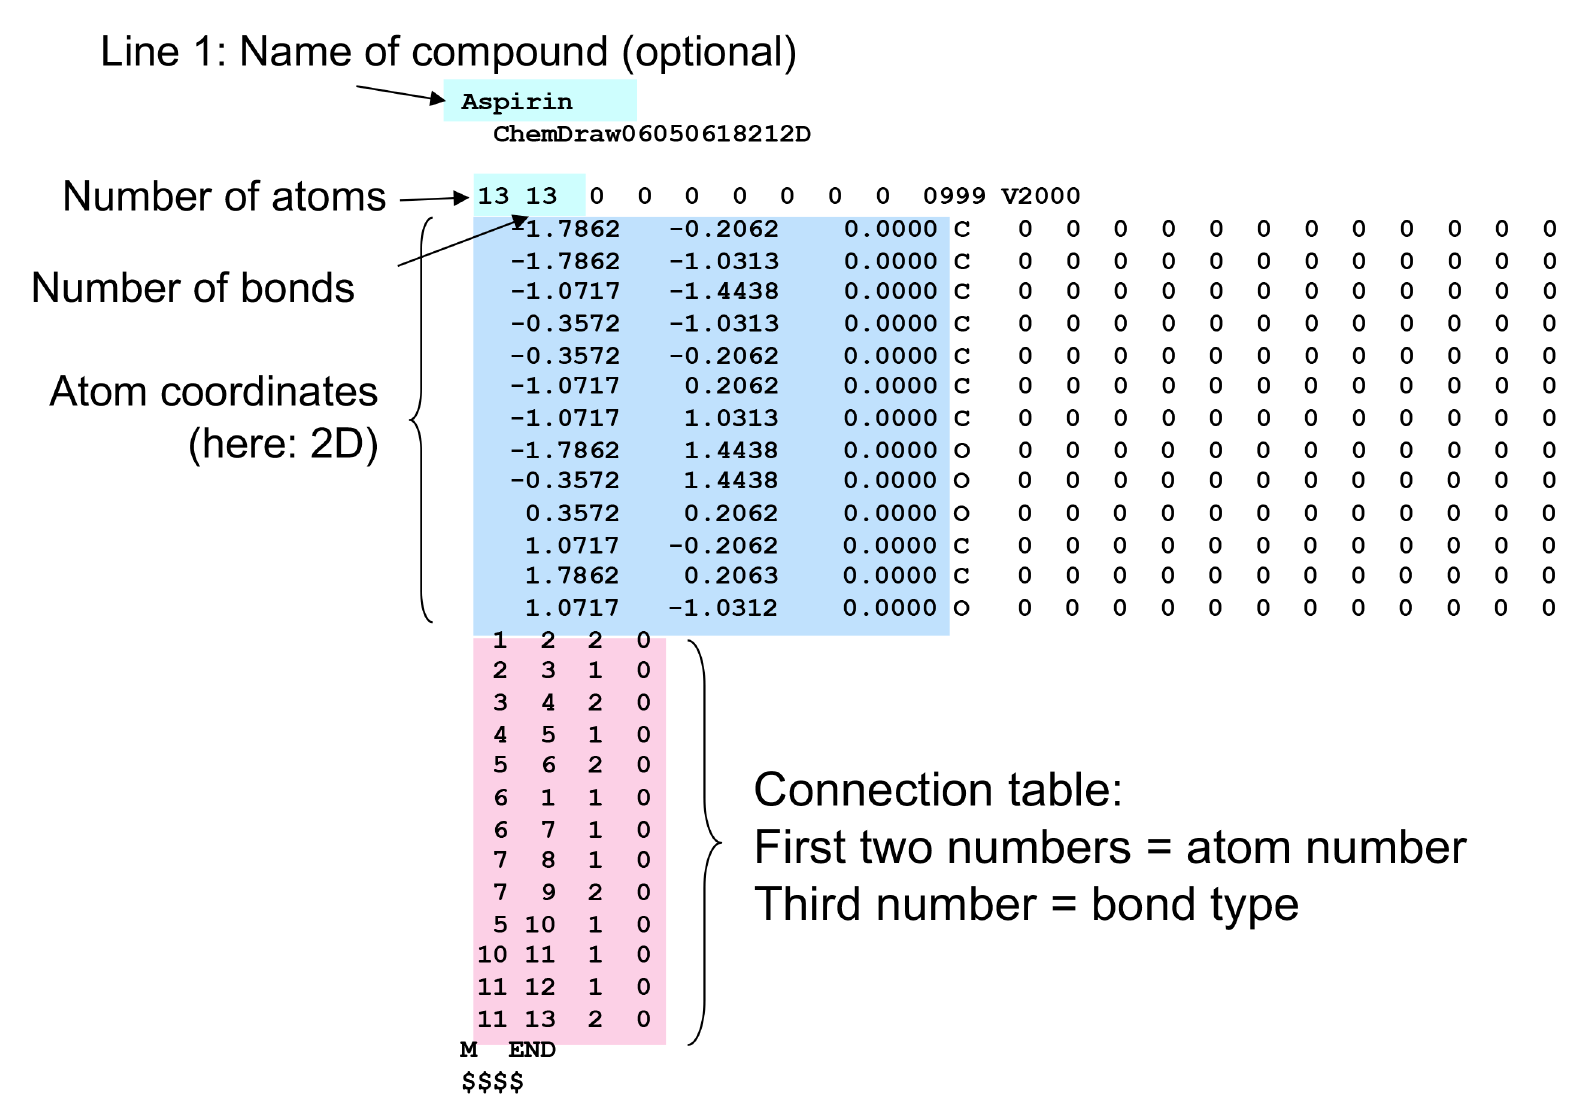
\includegraphics[width=0.70\textwidth]{img/cheminformatics/DataFormat.png}\end{center}

\subsection{1D representation}

The most efficient way to represent molecules for storage is a 1D representation. Furthermore, it can be easily interpreted by a computer and searched in a database. However, it is important that the representation is \emph{reversible}, that the transformations 2D $\rightarrow$ 1D and 1D $\rightarrow$ 2D can be carried out without any problems, and that the representation is \emph{unique}. To achieve this, stereochemistry and aromaticity must be retained in the representation. Examples of such representations are the IUPAC name, WLN, SLN, SMILES and InChI, although we will only deal with the latter two in the following.

\subsubsection{SMILES}

SMILES stands for \emph{Simplified Molecular Input Line Entry System}. It was introduced in 1988 and is based on representing the chemical structure using letters according to established rules. On the computer, a \emph{minimum spanning tree} is first created from a graph, which is then translated into the SMILES using a \emph{depth-first} algorithm, whereby different applicable SMILES are generated depending on which atom is started with. Therefore, a \emph{canonicalization} is needed to make the representation unique. SMILES follows the following rules:

\begin{itemize}
    \item Hydrogens as well as single and aromatic bonds are usually omitted, but can be specified explicitly if desired.
    \item \textbf{Atoms:}
    \begin{itemize}
        \item General: Atomic symbol in square brackets
        \item “Organic” subset (= B, C, N, O, P, S, F, Cl, Br, I) can be written without brackets if the number of attached Hs is “normal”.
        \item Attached hydrogens and formal charges always specified inside brackets.
        \item Atoms in aromatic rings are specified by lower case letters (i.e. c, n).
        \item Stereocentres are specified with @ (anti-clockwise writing of neighbors) and @@ (clockwise writing of neighbors) inside brackets.
    \end{itemize}
    \begin{center}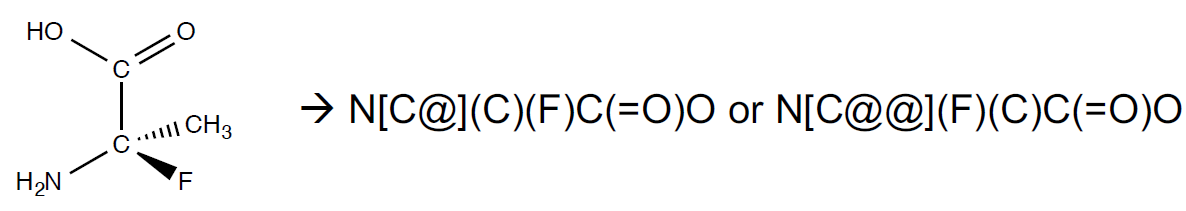
\includegraphics[width=0.65\textwidth]{img/cheminformatics/SmilesRulesAtoms.png}\end{center}
    \item \textbf{Bonds:}
    \begin{itemize}
        \item Single bond: “-”, double bond: “=“, triple bond: "\#" aromatic bond: “:”
        \item Cis/trans double bonds: use of “/” and “$\backslash$”, e.g.
    \end{itemize}
    \begin{center}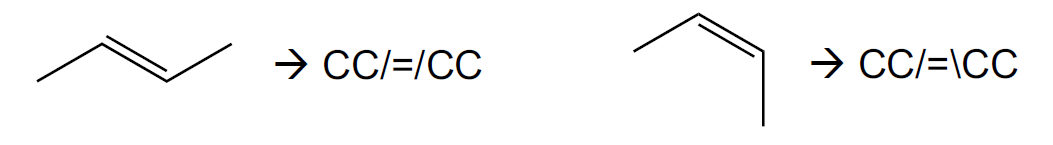
\includegraphics[width=0.65\textwidth]{img/cheminformatics/SmilesRulesBonds.png}\end{center}
    \item \textbf{Branches:}
    \begin{itemize}
        \item Specified by parentheses
        \item Can be nested or stacked
    \end{itemize}
    \begin{center}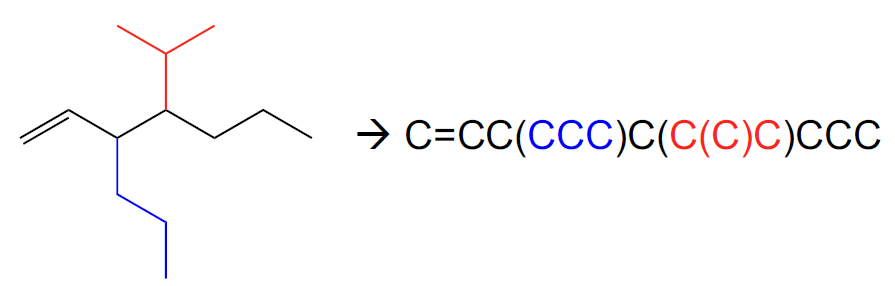
\includegraphics[width=0.65\textwidth]{img/cheminformatics/SmilesRulesBranches.png}\end{center}
    \item \textbf{Cyclic structures:}
    \begin{itemize}
        \item Represented by breaking one bond (to get spanning tree) and numbering the ring-closure atoms
        \item Ring-closure digits can be reused
    \end{itemize}
    \begin{center}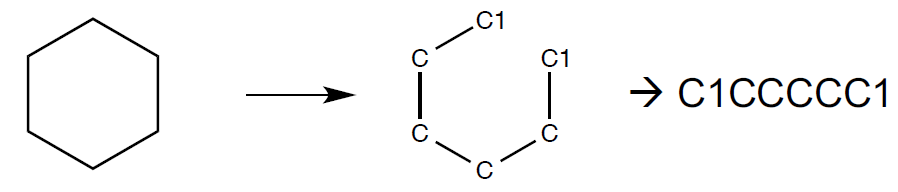
\includegraphics[width=0.65\textwidth]{img/cheminformatics/SmilesRulesCyclic.png}\end{center}
    \item \textbf{Aromaticity}
    \begin{itemize}
        \item Aromaticity in cheminformatics is a concept! Different definitions/algorithms exist (discussed later). Do not confuse it with a physical phenomenon
        \item Aromatic bonds are usually omitted
        \item Atoms in an aromatic ring are specified by lower case letters
    \end{itemize}
    \begin{center}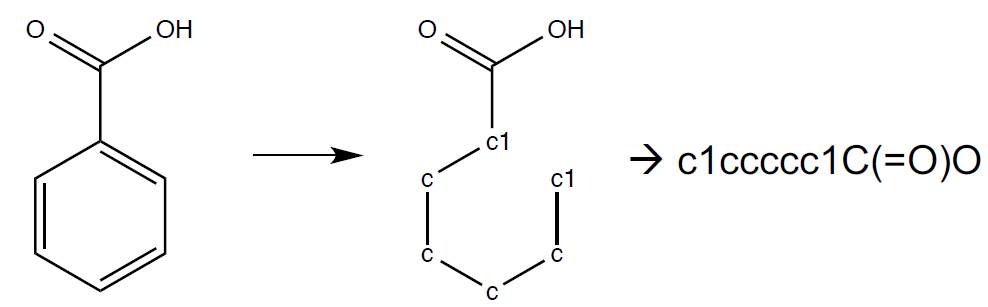
\includegraphics[width=0.65\textwidth]{img/cheminformatics/SmilesRulesAromaticity.png}\end{center}
\end{itemize}

\textcolor{red}{Beispiele aus den slides machen und einfügen.}

% not finished code
%\lstinputlisting[language=C++]{src/cheminformatics/smiles.cpp}

\subsubsection{Canonicalization}

As already mentioned, several correct SMILES can be used for one molecule, depending on which atom you start with. Therefore, a canonicalization must be performed to create a unique and reproducible numbering of the atoms of a molecule.

\deff{Graph Isomorphism}{Two graphs are isomorphic when there is a 1-to-1 mapping (a permutation) from the vertices of one graph to the vertices of the other, such that the edge connections are respected. In short, isomorphic graphs are structurally the same, but the labeling of the vertices is different.}

\deff{Graph Invariant}{In graph theory, a graph property or graph invariant is a property of graphs that depends only on the abstract structure, not on graph representations such as particular labellings or drawings of the graph. Therefore, two isomorphic graphs have the same invariants.}

In the example of cheminformatics, the invariants of a graph are usually a combination of information such as element, number of bonds, number of hydrogens, ring information, etc.

\paragraph{Morgan's Algorithm}
Morgan's algorithm is a canonicalization algorithm for chemical compounds presented in 1965 that uses the number of bonding partners (excluding hydrogen) as invariants. The algorithm proceeds as follows:

\begin{enumerate}
    \item \emph{Step 1: Find invariants}
    \begin{itemize}
        \item First assign the initial invariants to each atom, i.e. the number of bonds.
        \item Then assign new invariants for each atom, which are the sum of the invariants of the neighbors (excluding its own invariant). Repeat this step until the number of invariants no longer increases.
    \end{itemize}
    \begin{center}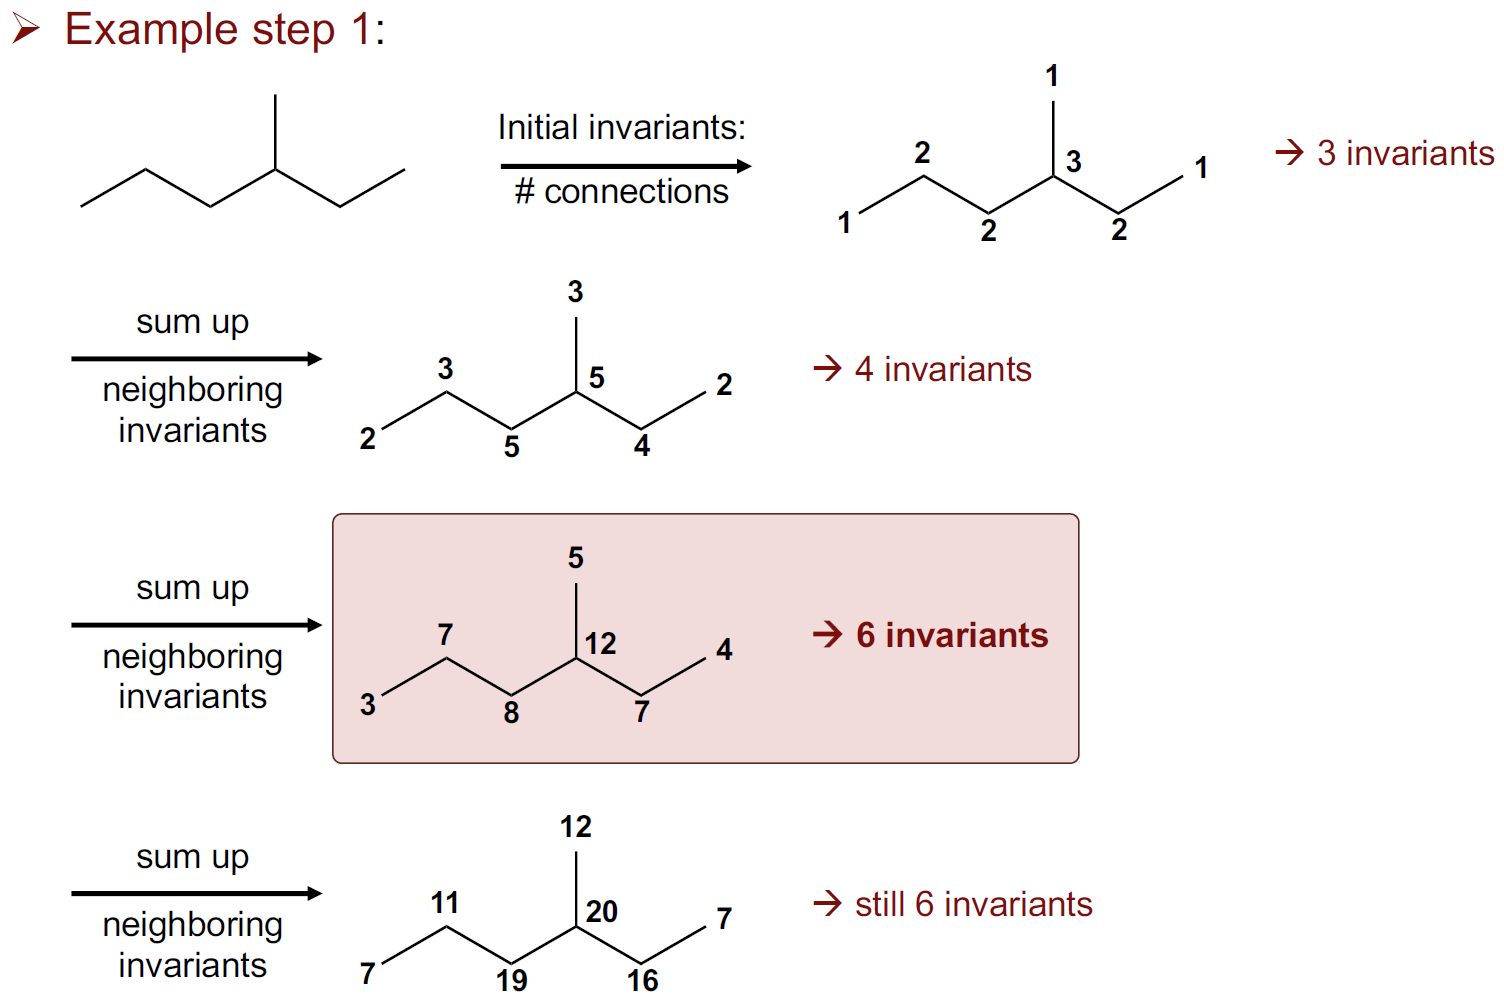
\includegraphics[width=0.85\textwidth]{img/cheminformatics/Morgan1.png}\end{center}
    \item \emph{Step 2: Set ranks}
    \begin{itemize}
        \item Take the graph where the number of invariants increased last time (not the graph where they were increased but the number of invariants remained the same).
        \item Take the largest invariant and set the rank of the atom to 1.
        \item Take the neighbors of the atom with rank 1, order them by descending invariants and give them the ranks 2-4 accordingly (assuming three are bonded).
        \item Now always choose the atom with the smallest rank and assign ranks to its neighbors according to descending invariants. Repeat this step until each atom has a rank.
    \end{itemize}
    \begin{center}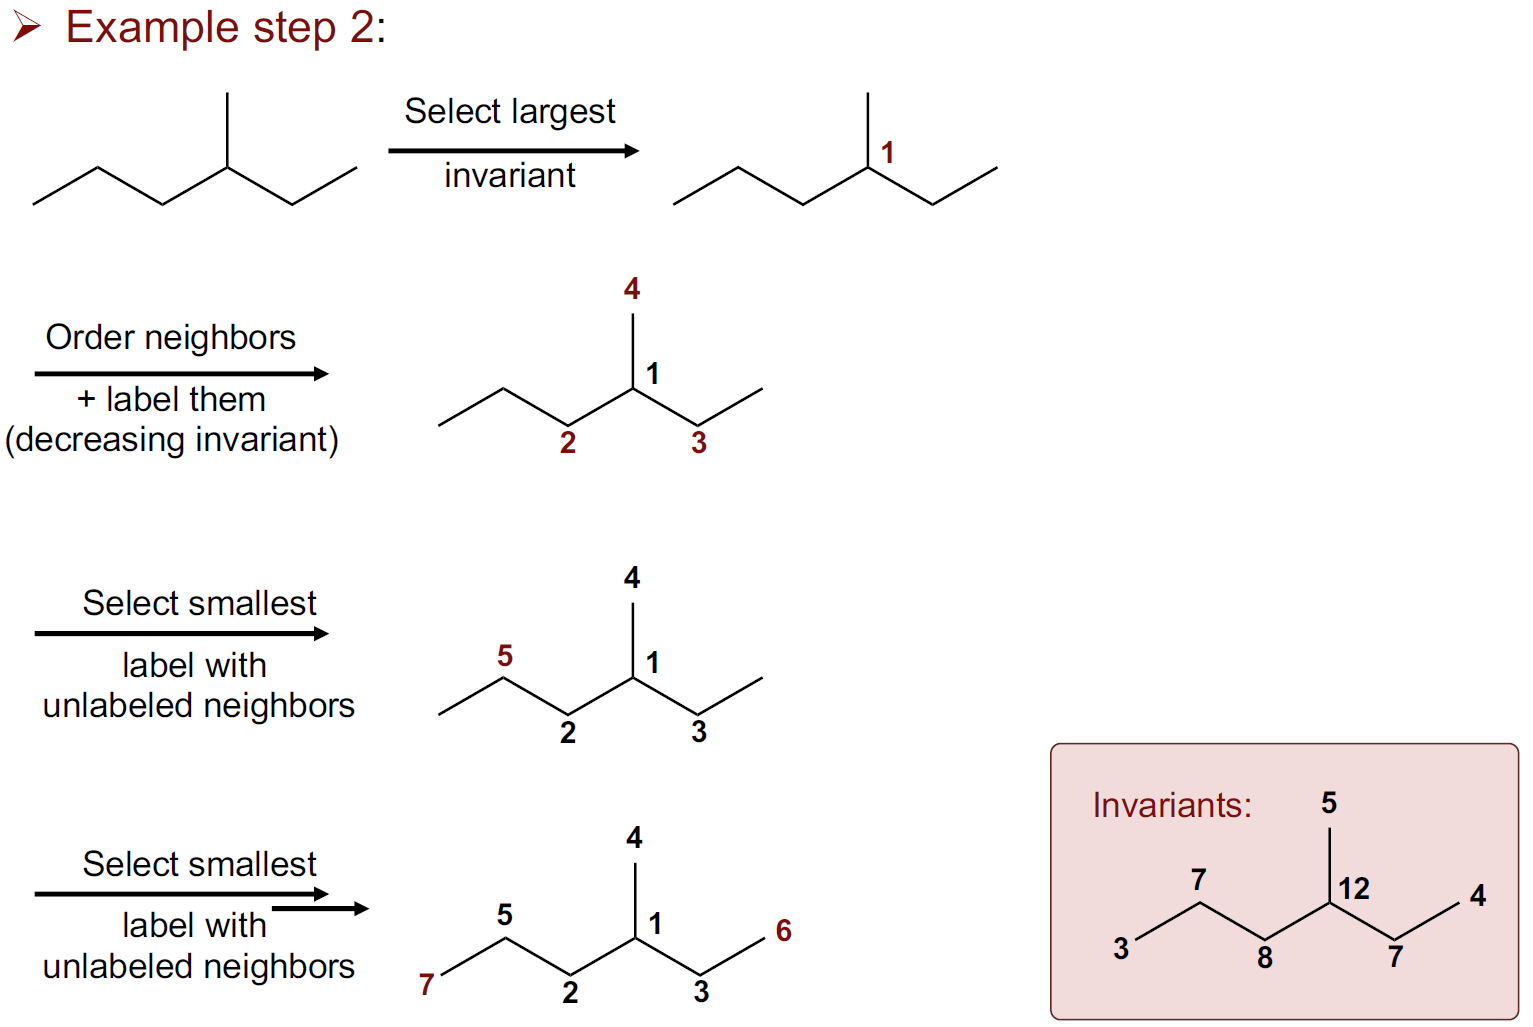
\includegraphics[width=0.85\textwidth]{img/cheminformatics/Morgan2.png}\end{center}
\end{enumerate}

The main criticism of Morgan's algorithm is that the summation step produces ambiguous results, which is why uniqueness cannot be proven. One way to solve this is to also include the atom type and bond multiplicity. Furthermore, oscillations can occur for certain symmetrical molecules, so that the first step has no termination condition.

% not finished code
%\lstinputlisting[language=C++]{src/cheminformatics/morgan.cpp}

\paragraph{Cangen Algorithm}

Just like Morgan's algorithm, CANGEN uses the number of binding partners to find the invariants. However, in the iterative calculation, CANGEN uses the product of primes instead of the sum of the invariants of the neighbors, as in Morgan's algorithm, to minimize ambiguities. However, a unique numbering cannot be proven here either.

\begin{enumerate}
    \item 
\end{enumerate}

% not finished code
%\lstinputlisting[language=C++]{src/cheminformatics/cangen.cpp}

\subsubsection{InChI}

\subsubsection{Ring perception}

The idea behind ring perception is to develop an algorithm that can automatically detect ring structures in 1D representations of molecules. The whole thing must therefore be independent of the projection, orientation and labeling of the ring system.

\begin{itemize}
    \item \textbf{Chords:}
    \begin{itemize}
        \item Minimum number of bonds whose removal is required to turn a structure from cyclic to acyclic.
    \end{itemize}
    \item \textbf{Nullity:}
    \begin{itemize}
        \item Number of chords that can be calculated using the formula below, where components stands for the number of closed graphs (always 1 for a molecule).
    \end{itemize}
    \begin{align}
        \mu=\#_\mathrm{bonds}-\#_\mathrm{atoms}+\#_\mathrm{components}
    \end{align}
    \item \textbf{Cycle:}
    \begin{itemize}
        \item Traversable node by node in a single path back to the start.
    \end{itemize}
\end{itemize}

The size we now want to determine exactly is the smallest set of smallest rings (SSSR), in which as many rings of the smallest possible size as possible are found. 

\begin{center}
    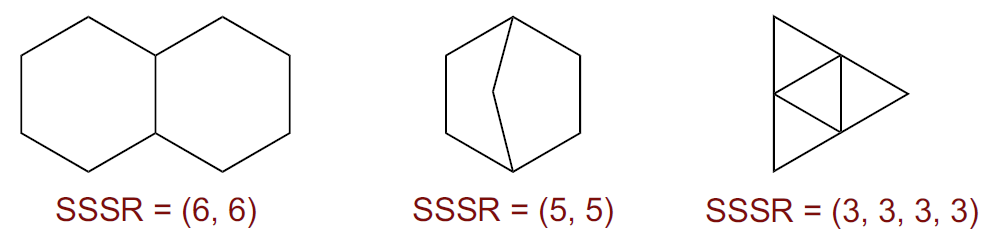
\includegraphics[width=0.85\textwidth]{img/cheminformatics/RingPerceptionSssr.png}
\end{center}

\paragraph{Figueras' algorithm}
Figueras' algorithm is an algorithm presented in 1996 to determine the SSSR of a molecule. The algorithm proceeds as follows:

\begin{enumerate}
    \item 
\end{enumerate}

\begin{center}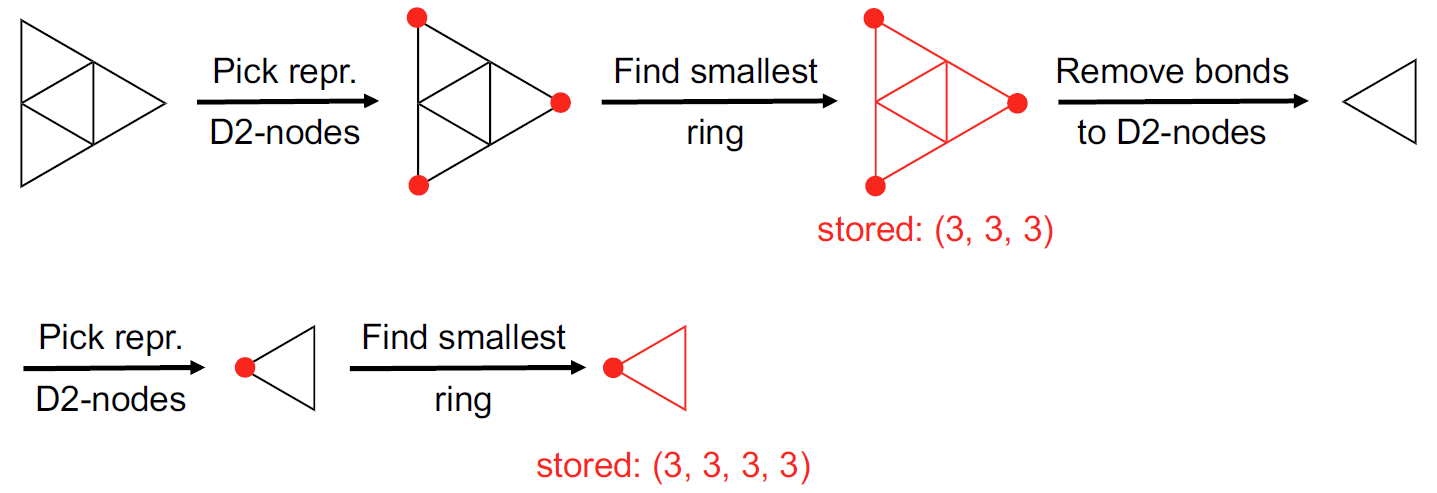
\includegraphics[width=0.85\textwidth]{img/cheminformatics/RingPerceptionFigueras1.png}\\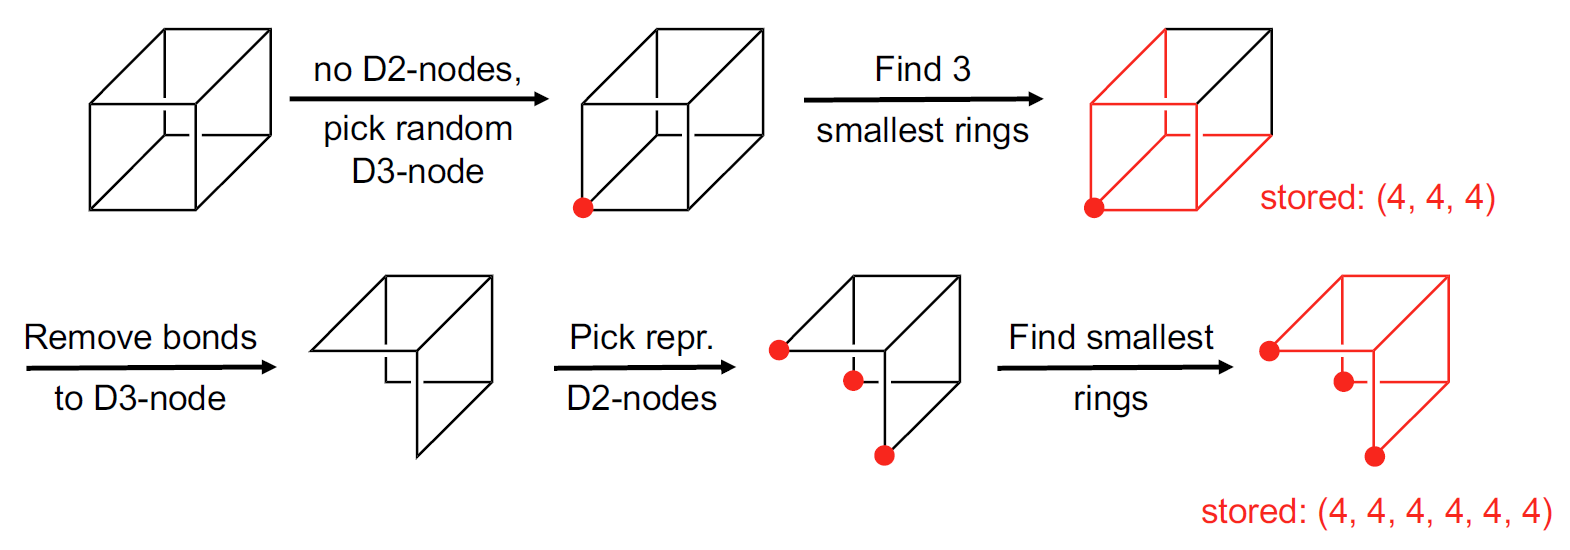
\includegraphics[width=0.85\textwidth]{img/cheminformatics/RingPerceptionFigueras2.png}\end{center}

% not finished code
%\lstinputlisting[language=C++]{src/cheminformatics/figueras.cpp}

\subsubsection{Aromaticity detection}

The definition of armoaticity is not trivial and the implementation in cheminformatics is still under discussion, because for cheminformatics a definition has to be found that is as simple as possible, that applies in most cases and is co-agent with SMILES and substructure search. Therefore, the cheminformatics definition does not necessarily imply physical properties of the molecule.

\begin{itemize}
    \item \textbf{Hückel's rule:}
    \begin{itemize}
        \item $(4n+2)\;\pi$-electrons $\rightarrow$ aromatic
    \end{itemize}
    \item \textbf{Extension of Hückel’s rule:}
    \begin{itemize}
        \item $(4n+2)\;\pi$-electrons and all atoms $\mathrm{sp}^2$ (planar) $\rightarrow$ aromatic
    \end{itemize}
\end{itemize}

With SMILES, both the Kekulè form (localized double bonds) can be used, as well as the explicit labeling of aromaticity with lowercase letters, whereby the latter is the preferred output of SMILES, since the former creates an artificial asymmetry.

\begin{align*}
    &\textit{Exapmle: benzene}&\begin{cases}
        \textit{Kekulè: }&\text{C1=CC=CC=C1}\\
        \textit{SMILES: }&\text{c1ccccc1}
    \end{cases}
\end{align*}

Aromatic systems over several rings are generally more difficult. For example, non-aromatic single bonds between two aromatic rings should be explicitly written with “-” in SMILES (e.g. biphenyl with c1ccccc1-c2ccccc2).

\paragraph{Aromaticity in the RDKit:}
The RDKit uses the Hückel rule for aromaticity, whereby a ring or condensed ring system with $(4n+2)\;\pi$-electrons is considered aromatic. Both bonds and atoms can be aromatic, whereby an aromatic bond must be between two aromatic atoms, but a bond between two aromatic atoms does not necessarily have to be aromatic. This is why in condensed ring systems the individual cycle can be not aromatic, but the overall system is.

\begin{center}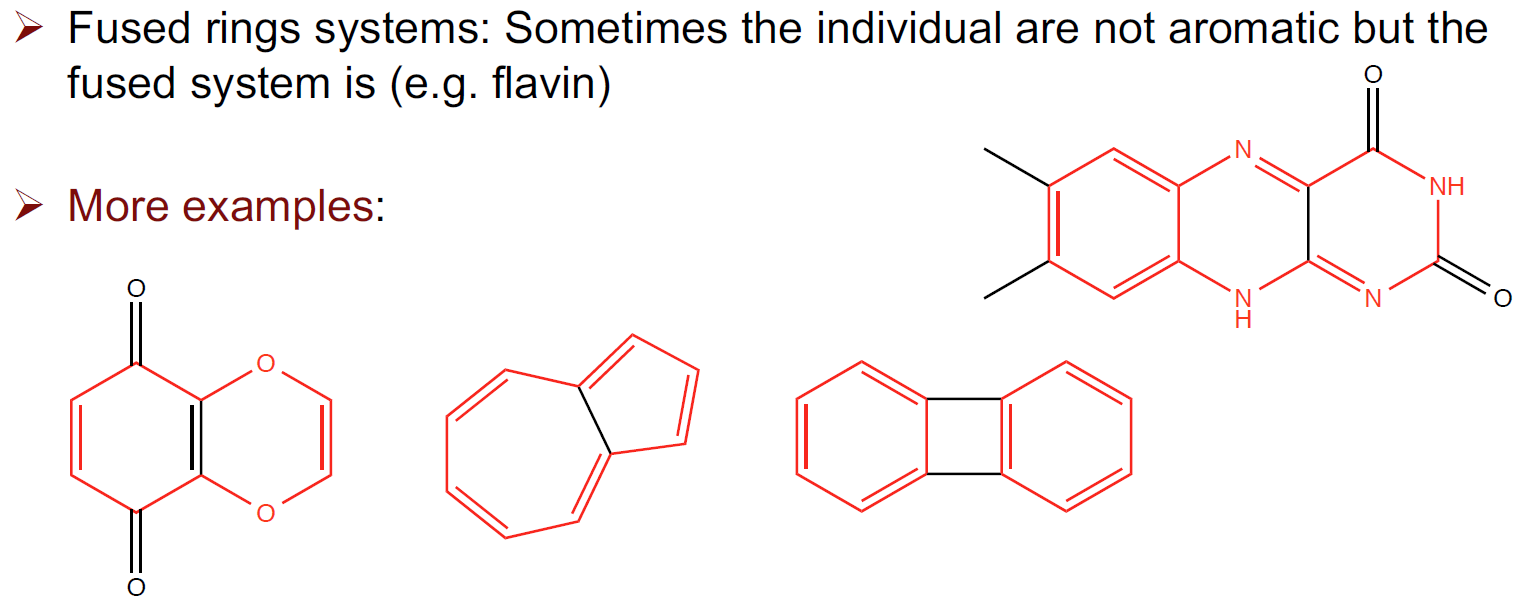
\includegraphics[width=0.85\textwidth]{img/cheminformatics/AromaticRdkit.png}\end{center}

\subsection{Substructure search}

In cheminformatics, a distinction is made between three shifting structure searches:

\begin{itemize}
    \item \textbf{Full structure search:}
    \begin{itemize}
        \item Question: Is this molecule in my database?
        \item Input: Full chemical structure (e.g. SMILES)
        \item Solution: Comparison of SMILES, InChi (keys), internal index number, etc.
    \end{itemize}
    \item \textbf{Substructure search:}
    \begin{itemize}
        \item Question: Does this substructure exist in any molecule of my database?
        \item Input: Query pattern of atoms and bonds (e.g. SMARTS).
        \item Solution: Brute-force, backtracking, partitioning and relaxation
    \end{itemize}
    \item \textbf{Superstructure search:}
    \begin{itemize}
        \item Question: Are any molecules in my database substructures of the query?
        \item Input: full chemical structure (e.g. SMILES)
        \item Solution: same as substructure search
    \end{itemize}
\end{itemize}

\subsubsection{SMARTS}

SMARTS (SMILES arbitrary target specification) is an extension of the classic SMILES to describe molecular patterns (substructures). With SMILES only exact atoms can be specified, whereas with SMARTS wildcards for atoms and bonds are possible, which can simplify the substructure search.

\begin{itemize}
    \item \emph{Atoms:}
    \begin{itemize}
        \item Specified by either element symbol or number: e.g. [\#6] $\rightarrow$ any carbon
        \item “*” : wild card
        \item “A” : any aliphatic atom
        \item “a” : any aromatic atom
        \item “D” followed by a number : degree (number of explicit connections)
        \item “R” followed by a number n : in n smallest rings
        \item “r” followed by a number n : in a smallest ring of size n
        \item “H” followed by a number : number of adjacent hydrogens
        \item H has now two meanings: e.g. [H] $\rightarrow$ hydrogen atom, [*H2] $\rightarrow$ any atom with two hydrogens
        \item Multiple possible matches are separated by a comma: e.g. [C,N] $\rightarrow$ either aliphatic C or N
    \end{itemize}
    \item \emph{Bonds:}
    \begin{itemize}
        \item “$\sim$” : any bond
        \item “@” : any ring bond
    \end{itemize}
    \item \emph{Logical operators:} combinations of atom and bond specifications
    \begin{itemize}
        \item “!” : NOT, e.g. [!C] $\rightarrow$ not aliphatic carbon
        \item “\&” : AND (high priority)
        \item “,” : OR
        \item “;” : AND (low priority)
        \item Operator priority: “!” > “\&” > “,” > “;”
    \end{itemize}
    \item \emph{Aromaticity:}
    \begin{itemize}
        \item Note: a double bond is not matched to an aromatic bond!
    \end{itemize}
\end{itemize}

\begin{center}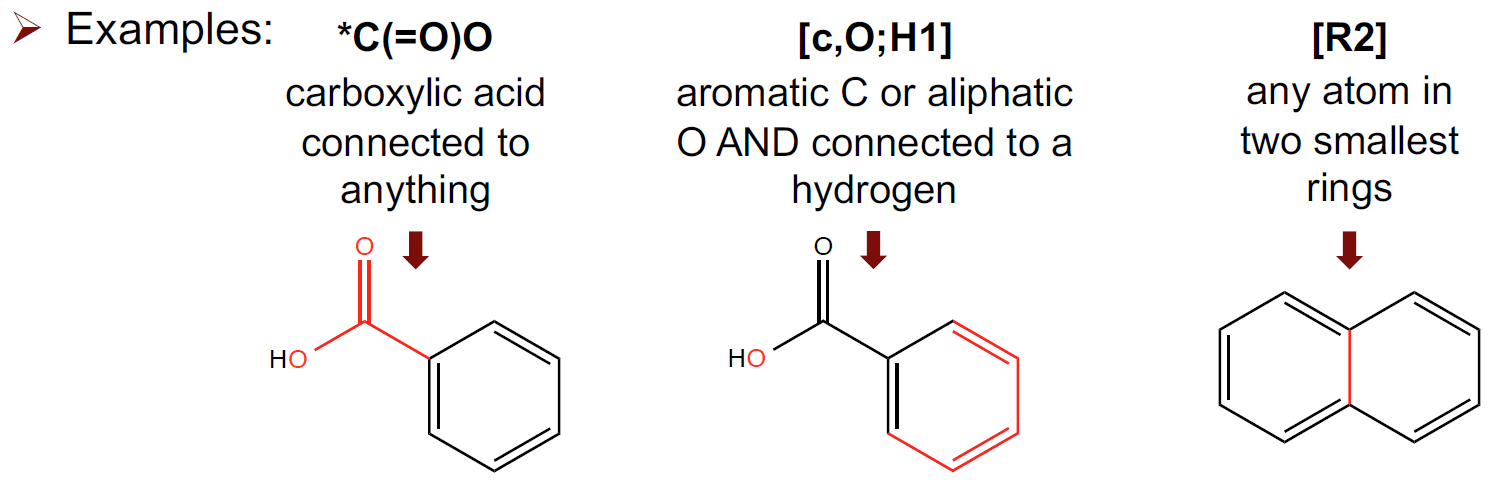
\includegraphics[width=0.85\textwidth]{img/cheminformatics/SubstructureSmartsExample.png}\end{center}

Algorithmically, however, such a search is not easy to program. If we consider the problem of checking whether two graphs are isomorphic, this algorithm already scales with $\Theta(N!)$, where $N$ is the number of nodes in the graph. In this brute-force algorithm (depth-first tree search), a 1-to-1 mapping is made so that each node from $G_1$ is mapped against an unmapped node from $G_2$ and it is checked whether all neighbors are equal. It is assumed that graph isomorphism is an \emph{NP-complete} problem, but this has not yet been proven rigerously.

\deff{Subgraph isomorphism}{The subgraph isomorphism problem is a generalization of graph isomorphism, where the question is whether $G_1$ is a subgraph of $G_2$. In the worst case this is an NP-complete problem, but average running time is much better than for the classical graph isomorphism problem. In addition, heuristics can be used for molecular graphs, which also reduce the running time (bounded valence and bond multiplicity)}

In general, there are the following algorithms for substructure search:

\begin{itemize}
    \item \emph{Backtracking}
    \begin{itemize}
        \item Rax and Kirsch \shortrefurl{Science}{1975}{126}{814-819}{https://doi.org/10.1126/science.126.3278.814}
    \end{itemize}
    \item \emph{Partitioning and relaxation (often combined with backtracking)}
    \begin{itemize}
        \item Sussenguth’s partitioning algorithm \shortrefurl{J. Chem. Docum.}{1965}{5}{36-43}{}
        \item Figueras’ set reduction algorithm \shortrefurl{J. Chem. Docum.}{1972}{12}{237-244}{}
        \item Ullmann’s algorithm \shortrefurl{J. Assoc. Comput. Mach.}{1976}{23}{31-42}{}
        \item von Scholley’s relaxation algorithm \shortrefurl{J. Chem. Inf. Comput. Sci.}{1984}{24}{235-241}{}
        \item vf2 and variants \shortrefurl{IEEE Trans Pattern Analysis Machine Intelligence}{2004}{26}{1367-1372}{}
    \end{itemize}
\end{itemize}

In the worst case, the running time is still exponential, but that doesn't happen often.

\subsubsection{Backtracking (Ray and Kirsch)}

Backtracking uses a depth first algorithm (for the searching tree) to map one graph of the pattern (substructure) against the graph of the full molecule. As soon as a branch is no longer possible, it is backtracked to an atom where a solution is still possible.

\begin{enumerate}
    \item Map arbitrary pair of nodes.
    \item Map neighbors of these nodes.
    \item If successful repeat step 2, if not backtrack to step 1 and choose another pair (query atom stays the same).
\end{enumerate}

The algorithm is terminated when either all atoms of the pattern have been successfully mapped (MATCH) or all mapping attempts of the first query node fail (NO MATCH). You can speed up the algorithm somewhat by, for example, only mapping nodes with the same element, charge and number of bonds against each other, or by starting with unusual atoms with many bonds, because then the probability of recognizing a mismatch earlier is higher.

\begin{center}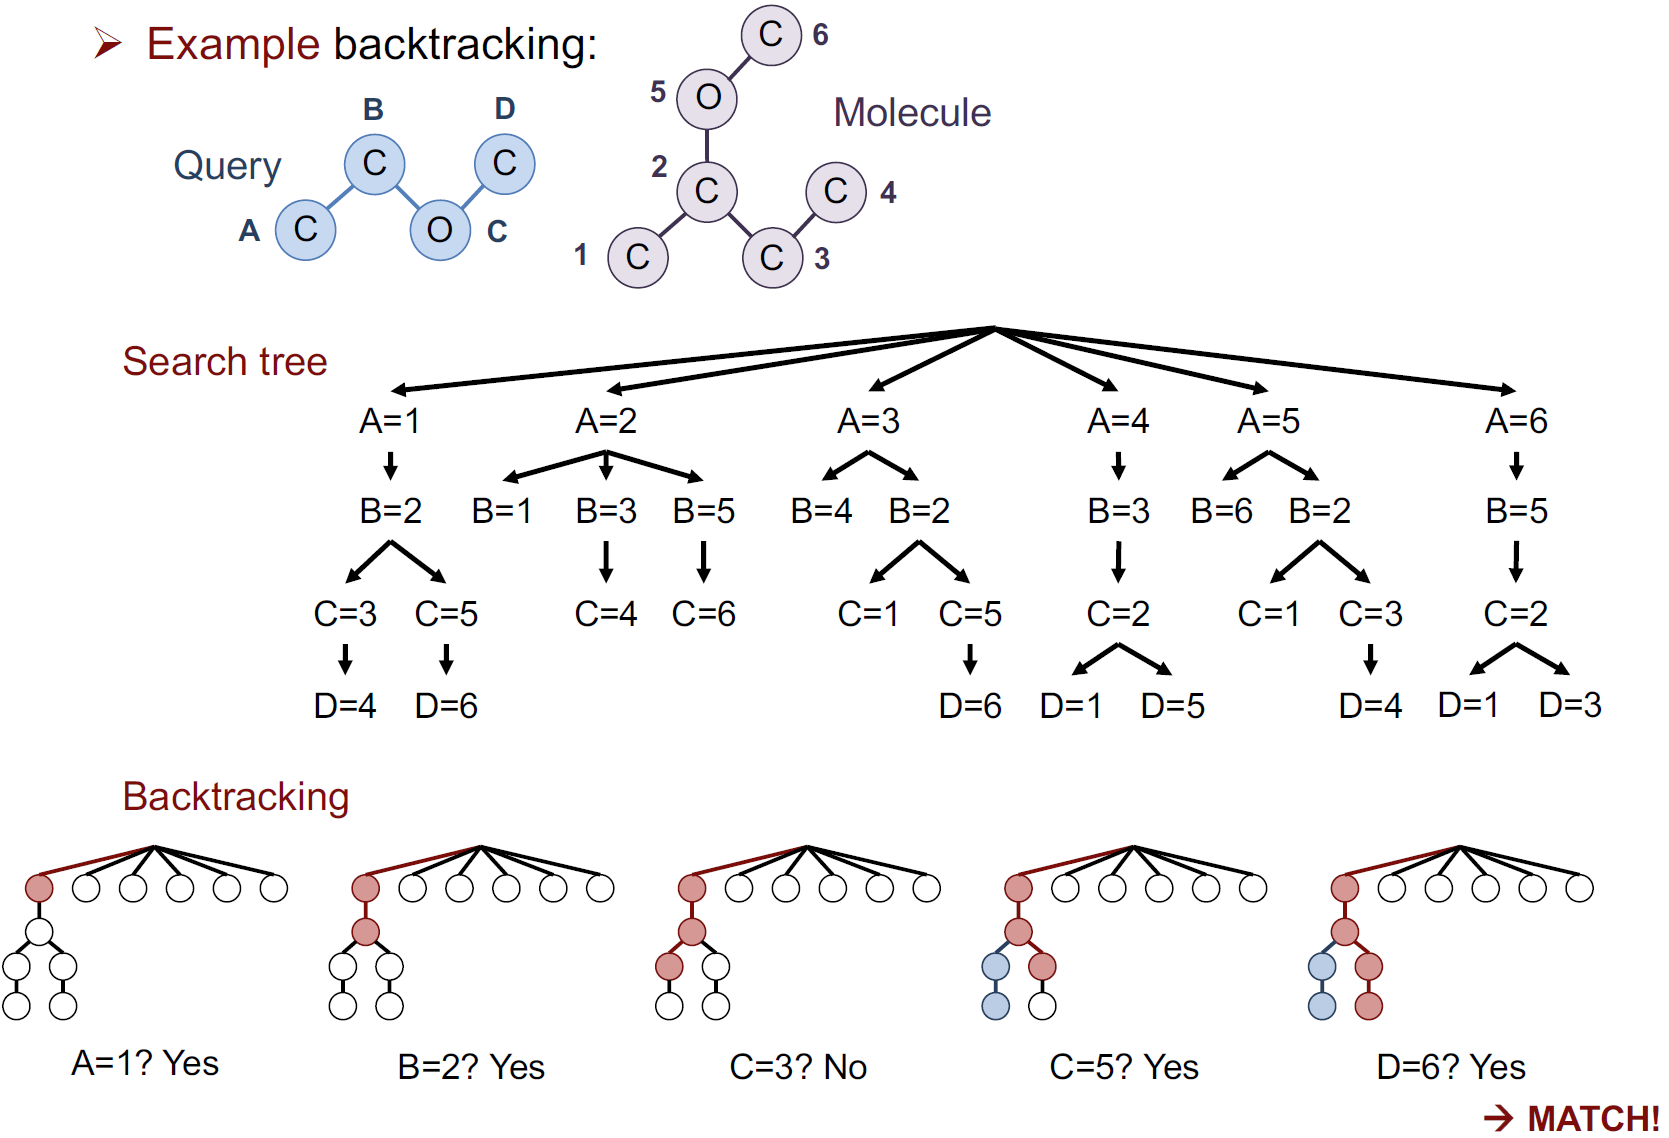
\includegraphics[width=0.85\textwidth]{img/cheminformatics/SubstructureBacktracking.png}\end{center}

\subsubsection{Partitioning and relaxation (Ullmann's algorithm)}

\subsubsection{Molecular fingerprints}

\subsection{Chemical reactions}

\subsection{Dimensionality reduction}

\subsection{Fingerprints}

\subsection{Maximum common substructure}

\subsection{Scaffolds}

\subsection{Generation of 3D coordinates}

\subsubsection{Distance geometry}

\subsection{Clustering}

\subsubsection{Hierarchical}

\subsubsection{Application to chemical space}

\subsubsection{Non-hierarchical}

\subsubsection{Application to conformations}

% tex: nichts
% src: nichts
\newpage\section{Introduction to Machine-Learning}% Introduction to Machine-Learning (1 week)

%\lstinputlisting[language=C++]{src/intro/test.cpp}

The idea behind \emph{supervised machine learning} is to determine a function from a set of training data that can be used to predict the output of new data. The training data is a representative set of examples with input values (typically a vector) and a known output value. Typical machine learning tasks are, for example, \emph{classifications} (discrete output: for example, a molecule is biologically active or not) or \emph{regressions} (continuous output: for example, linear regression).

\begin{center}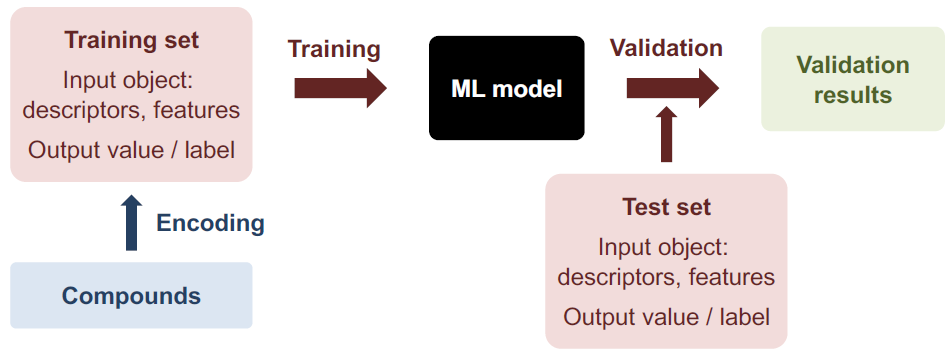
\includegraphics[width=0.65\textwidth]{img/machine/MachineGeneralScheme.png}\end{center}

The following methods, among others, can be used for this purpose:

\begin{itemize}
    \item Linear models, e.g. linear regression, logistic regression
    \item Decision tree
    \item Random forest
    \item Gradient tree boosting
    \item Naïve Bayes
    \item Support vector machines (SVM)
    \item Artificial neural networks
\end{itemize}

\paragraph{Validation}
Once a function has been determined from the training data, it still needs to be validated, since the training data for such algorithms is often too small and there is a risk of overfitting the training data, whereby the function performs well on the training set but not well on new data. Typical validation techniques are \emph{train/test split} or \emph{K-fold cross-validation}.

\begin{center}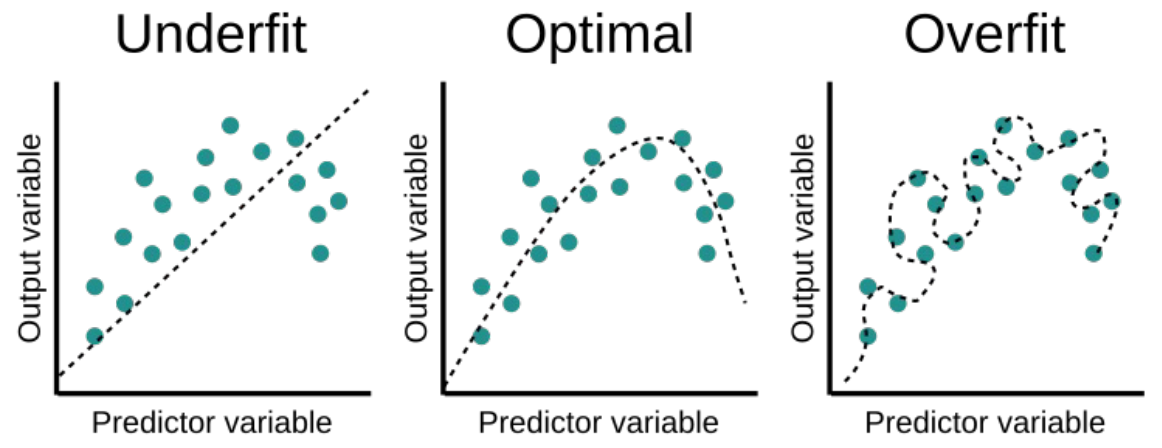
\includegraphics[width=0.65\textwidth]{img/machine/MachineOverUnderFiting.png}\end{center}

For classification models, slightly different assessment criteria for the quality of an ML-model must be applied, such as the \emph{receiver-operator curve} (ROC), in which the true positive rate is plotted against the false positive rate. Depending on the error rates, further metrices for classification models can be calculated.

\begin{center}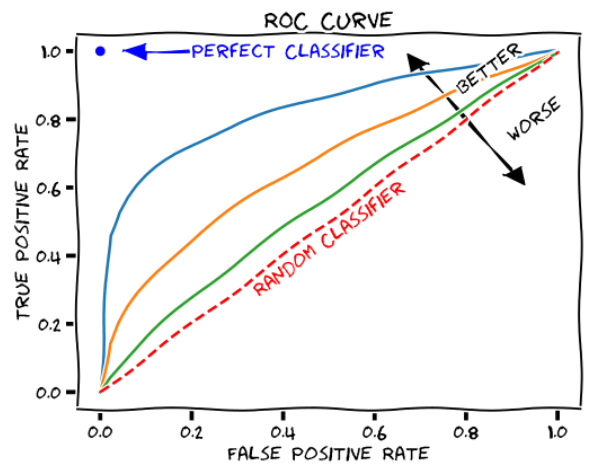
\includegraphics[width=0.45\textwidth]{img/machine/MachineRocCurve.png}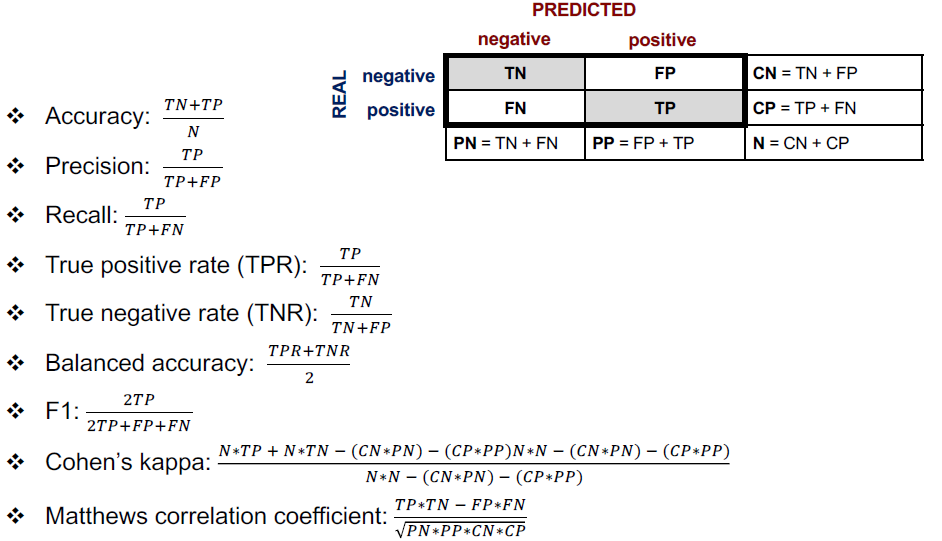
\includegraphics[width=0.45\textwidth]{img/machine/MachineClassificationMetrices.png}\end{center}

\paragraph{Unsupervised Machine Learning vs Supervised Machine Learning}
The difference between supervised machine learning and unsupervised machine learning is that in unsupervised machine learning the dataset does not yet have any labels without predefined patterns according to which the data is sorted. An example of this is clustering. In supervised machine learning, training data is used to determine a function.

\subsection{Linear models: linear regression, logistic regression}

\paragraph{Linear Regression}
Linear regression is the simplest ML-model and has as training data a set of example values of $(x,y)$ values, where the input values are the $x$ values and the output values (continues) are the $y$ values. The goal of the regression is to find a linear function $y(x)=ax+b$ for which the squared distances of the points from the regression line are minimized. 

\paragraph{Logistic Regression}
In logistic regression (similar to multiple linear regression), an input vector $X_i=(x_{1,i}, x_{2,i},\cdots,x_{N,i})$ is compared to a discrete output value $Y$ (here either 0 or 1, but generally classification) as training data. The coefficients $(a_1,a_2,\cdots,a_N)$ are fitted for a logistic function, where $p_i$ is the probability for a $y$-value. These models are often relatively simple but very effective.

\begin{align}
    \log_{2}\left(\frac{p_i}{1-p_i}\right)=a_0+a_1x_{1,i}+\cdots+a_Nx_{N,i}
\end{align}

\begin{center}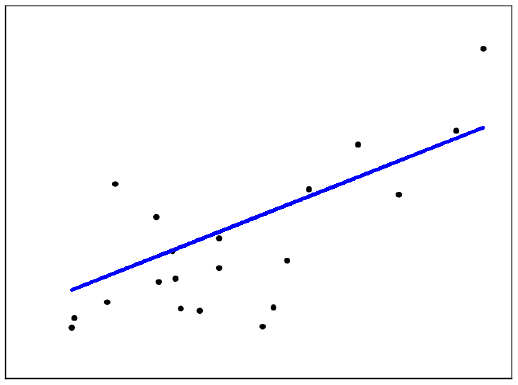
\includegraphics[width=0.35\textwidth]{img/machine/MachineLinearRegression.png}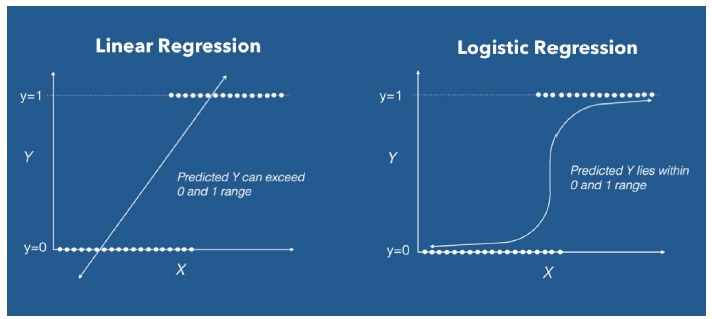
\includegraphics[width=0.55\textwidth]{img/machine/MachineLogisticRegression.png}\end{center}

\subsection{Decision trees}

\emph{Decision trees} can be used in machine learning for both classifications and regressions. They use as training data as input variable vectors with multiple attributes and as output variables integer or continuous values. The attributes of the input vector determine which branch of the decision tree is taken.

\begin{center}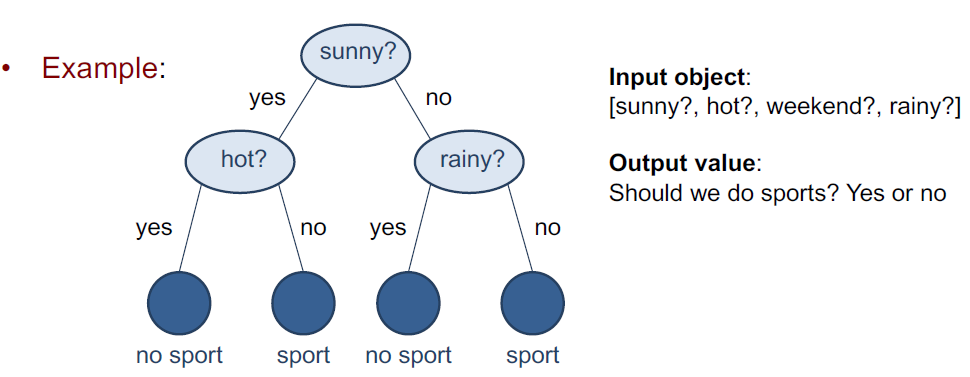
\includegraphics[width=0.65\textwidth]{img/machine/MachineDecisionTrees.png}\end{center}

In decision trees, the selection of attributes that are responsible for the splitting at the nodes is crucial. You set up the tree so that you get the maximum amount of information at each decision point, which is synonymous with reducing entropy/impurity. Where $p_{x,i}$ is the probability for the value $i$ for the attribute $x$, $N$ is the number of samples and $n$ is the number of attribute values.

\begin{align}
    &S(x)=\left(-p_{x,A}\log_2p_{x,A}\right)+\left(-p_{x,I}\log_2p_{x,I}\right)&Gain(x_2)=S(x_1)-\sum_{i=1}^{n}\frac{N_{x_2,\mathrm{tot}}}{N_{x_1,\mathrm{tot}}}S(x_2,i)
\end{align}

\begin{center}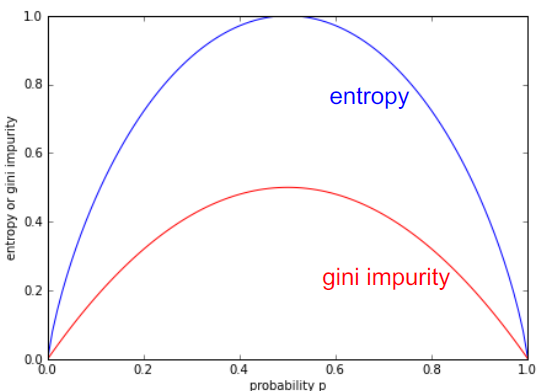
\includegraphics[width=0.65\textwidth]{img/machine/MachineDecisionTreesEntropy.png}\end{center}

\deff{Gini impurity}{Gini impurity measures how often a randomly chosen element of a set would be incorrectly labeled if it were labeled randomly and independently according to the distribution of labels in the set. It reaches its minimum (zero) when all cases in the node fall into a single target category.}

\begin{center}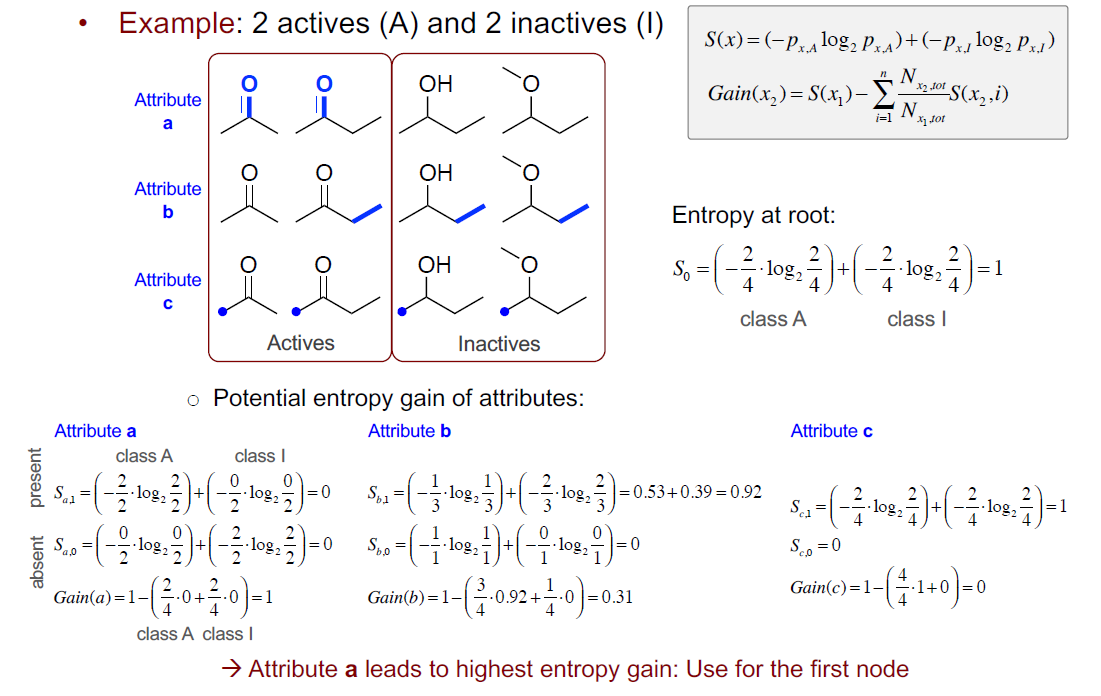
\includegraphics[width=0.65\textwidth]{img/machine/MachineDecisionTreesEntropyExample.png}\end{center}

The advantages and disadvantages of decision trees for machine learning are listed below:

\begin{itemize}
    \item[$\oplus$] Simple to understand and easy to interpret
    \item[$\oplus$] Little data preparation needed
    \item[$\oplus$] Both classification and regression possible
    \item[$\oplus$] Validation using statistical tests possible: Reliability of the model can be accounted for
    \item[$\ominus$] Prone to overfitting: Over-complex trees that do not generalise well (remedies: Pruning, limit maximum depth)
    \item[$\ominus$] Small variations in the data can lead to completely different trees
    \item[$\ominus$] Problem of learning an optimal decision tree is NP-complete (heuristic (greedy) algorithms required)
    \item[$\ominus$] If the training data is unbalanced, the resulting trees will be biased
\end{itemize}

\subsection{Ensemble methods}

The idea behind \emph{ensemble learning} is that you use the results of many not-so-strong models to achieve a strong overall result, which is then comparable to the wisdom of the crowd. For example, this is the case when several smaller decision trees only have a random subset of the training data and the output is decided by the majority of the individual models. The biggest advantage is that these models are usually more robust and the data that was not used by the individual trees can be used immediately as validation.

\begin{center}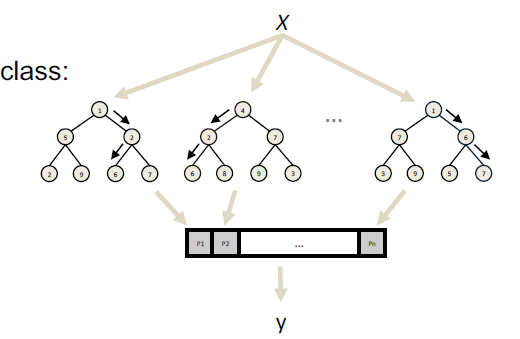
\includegraphics[width=0.65\textwidth]{img/machine/MachineEnsemble.png}\end{center}

\subsubsection{Random Forests}

Random Forests is an ensemble method that introduces a second random element (on the one hand, a random subset of training data per tree and, on the other hand, a random subset of attributes per node) to develop even more robust machine learning models. The first application for drug design of RFs was for quantitative structure-activity relationship models.

\begin{center}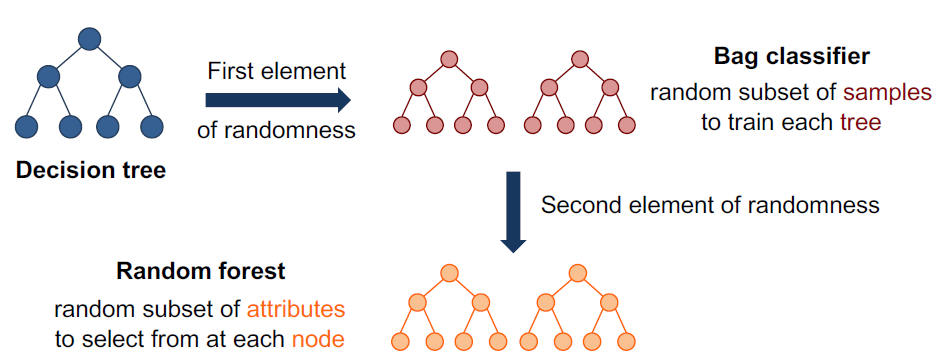
\includegraphics[width=0.65\textwidth]{img/machine/MachineEnsembleRandomForests.png}\end{center}

\subsubsection{Gradient Tree Boosting}

Gradient tree boosting is an ensemble method that is very similar to random forests, but here the trees are created sequentially after the training data has been run through, so that this information can be used to create better trees and thus make even better models than RFs, but the implementation usually takes longer.

\begin{center}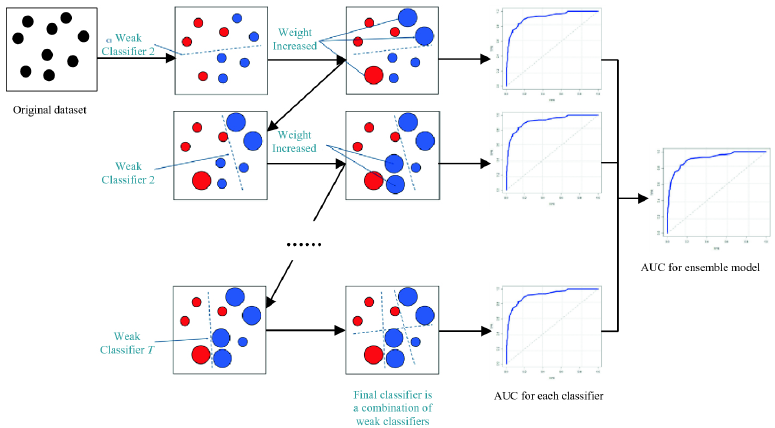
\includegraphics[width=0.65\textwidth]{img/machine/MachineEnsembleGradientTreeBoosting.png}\end{center}

\subsection{Artificial neural networks}

\deff{Artificial neuron}{The artificial neuron is the basic unit of information reception where the inputs are received and multiplied, summed, and processed via a transfer function before being delivered to the output.}

Here $f()$ is the transfer function, $b$ is the external error, the weights $w_{ij}$ are determined by the training and $a()$ is the decision function. This model always requires a training and a validation set.

\begin{align}
    y_i=f\left(\sum_{j=1}^{n}w_{ij}x_j+b\right)
\end{align}

\begin{center}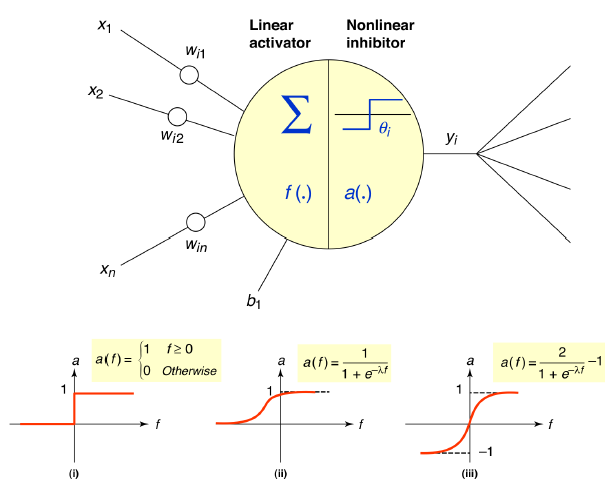
\includegraphics[width=0.65\textwidth]{img/machine/MachineArtificialNeuralNetworks.png}\end{center}

\subsection{Practical Considerations}

\begin{itemize}
    \item \textbf{Imbalanced datasets}
    \begin{itemize}
        \item Very common situation
        \item Diverse methods to address it, e.g. random undersampling of majority class, oversampling of minority class or threshold shifting
    \end{itemize}
    \item \textbf{Splitting of dataset into training and test sets}
    \begin{itemize}
        \item Random (should be repeated multiple times)
        \item Cluster based, e.g. move all compounds with the same scaffold either into training or testing
        \item Time splits
    \end{itemize}
    \item \textbf{Model interpretability}
    \begin{itemize}
        \item Random forests: Feature importances
    \end{itemize}
    \item \textbf{Applicability domain}
    \begin{itemize}
        \item Defined by the scope of the training set
        \item Models good at interpolation, true extrapolation very difficult
    \end{itemize}
\end{itemize}

% tex: nichts
% src: nichts
\newpage\section{Algorithms in Bioinformatics}% Algorithms in Bioinformatics

test

%\lstinputlisting[language=C++]{src/intro/test.cpp}

\end{document}
